\chapter{来自抗碰撞哈希的消息完整性}\label{chap:8}

在上一章中,我们讨论了通用哈希函数 (UHF),并且展示了如何使用通用哈希函数来构建 MAC。回顾一下,UHF 是\emph{带密钥}的哈希函数,只要密钥被秘密地保存,找到哈希的碰撞就是困难的。

在本章中,我们将研究\emph{无密钥}的哈希函数,对于它们来说,找到哈希碰撞仍然是困难的。非正式地说,一个无密钥函数就是一个可有效计算的,描述完全公开的函数。它没有任何密钥,并且任何人都可以评估该函数。令 $H$ 是一个无密钥哈希函数,它将某个大的消息空间 $\mathcal{M}$ 上的元素哈希为某个小的摘要空间 $\mathcal{T}$ 上的元素。与上一章一样,当:
\[
H(m_0)=H(m_1)
\quad\text{and}\quad
m_0\neq m_1
\]
时,我们就称两条消息 $m_0,m_1\in\mathcal{M}$ 是函数 $H$ 的一个\textbf{碰撞(collision)}。非正式地说,如果找到一个 $H$ 的碰撞是困难的,我们就称函数 $H$ 是\textbf{抗碰撞的(collision resistant)}。由于摘要空间 $\mathcal{T}$ 比消息空间 $\mathcal{M}$ 要小得多,所以我们知道,其实是存在许多这样的碰撞的。尽管如此,如果 $H$ 是抗碰撞的,那么实际上找到一个碰撞的数对 $m0,m1$ 应该是很困难的。我们将在下一节中给出一个更精确的定义。

在这一章中,我们将构造抗碰撞的函数,并介绍一些它的应用。为了举一个抗碰撞函数的例子,我们会介绍一个美国联邦标准,称作安全哈希算法标准,简称为 SHA。SHA 标准描述了一些能够提供不同程度的抗碰撞性能的哈希函数。例如,\textbf{SHA256} 是一个能将长消息哈希成 $256$ 比特摘要的函数。我们相信,找到 SHA256 的碰撞是很困难的。

抗碰撞哈希函数有许多应用。我们在这里简要介绍两个这样的应用,并在本章的稍后部分给出更多细节。本书的其他部分还会涉及到更多的应用。

\begin{snote}[扩展密码学原语。]
抗碰撞性的一个重要应用是它能够将为短输入建立的原语扩展成为更长输入建立的原语。我们举一个 MAC 构造作为例子。假设我们被给定一个 MAC 系统 $\mathcal{I}=(S,V)$,它只能认证短的消息,比如说 $256$ 比特长的消息。我们想扩展 MAC 的域,使其能够验证更长的消息输入。抗碰撞哈希给出了一个非常简单的解决方案。为了计算某个长消息 $m$ 的 MAC,我们可以先对 $m$ 进行哈希,然后将 $S$ 应用在所得到的短摘要上,如图 \ref{fig:8-1} 所示。换句话说,我们实际上定义了一个新的 MAC 系统 $\mathcal{I}=(S',V')$,其中 $S'(k,m):=S\big(k,H(m)\big)$。MAC 验证的工作方式与此类似,我们首先对消息进行哈希,然后验证摘要的标签。

显然,如果找到 $H$ 的碰撞是容易的,这种先哈希后 MAC 的构造就不安全了。如果对手能找到两条长消息 $m_0$ 和 $m_1$ 使得 $H(m_0)=H(m_1)$,那么它就可以用选择消息攻击来伪造标签。假设 $m_0$ 是一条无害的消息,但 $m_1$ 是恶意的内容,比如一个被病毒感染的程序。对手会请求消息 $m_0$ 的标签,并得到一个标签 $t$ 作为应答。那么这个数对 $(m_0,t)$ 就是一个有效的消息-标签对,但是数对 $(m_1,t)$ 同样也是有效的。因此,对手能够为 $m_1$ 伪造一个标签,这就破坏了 MAC。更糟糕的是,有效的标签可能会欺骗用户运行病毒。这个论证表明,抗碰撞性是这种先哈希后 MAC 构造满足安全性的必要条件。在本章的稍后部分,我们将证明抗碰撞性实际上足以证明安全性。

\begin{figure}
	\centering
	\tikzset{every picture/.style={line width=0.75pt}}

\begin{tikzpicture}[x=0.75pt,y=0.75pt,yscale=-1,xscale=1]

\draw  [fill={rgb, 255:red, 255; green, 255; blue, 255 }  ,fill opacity=1 ][line width=1.2] [general shadow={fill=black,shadow xshift=2.25pt,shadow yshift=-2.25pt}] (180,50) -- (220,50) -- (220,90) -- (180,90) -- cycle ;
\draw  [fill={rgb, 255:red, 255; green, 255; blue, 255 }  ,fill opacity=1 ][line width=1.2] [general shadow={fill=black,shadow xshift=2.25pt,shadow yshift=-2.25pt}] (70,40) -- (120,59.07) -- (120,80.93) -- (70,100) -- cycle ;

\draw  [->]  (220,70) -- (280,70) ;
\draw  [->]  (120,70) -- (179,70) ;
\draw  [->]  (0,70) -- (69,70) ;
\draw  [->]  (200,0) -- (200,49) ;
\draw  [->]  (200,55) -- (196.5,50) -- (203.5,50) -- cycle ;

\draw (280,66.6) node [anchor=south] [inner sep=0.75pt]    {$t$};
\draw (2,66.6) node [anchor=south west] [inner sep=0.75pt]    {$m$};
\draw (202,3.4) node [anchor=north west][inner sep=0.75pt]    {$k$};
\draw (95,70) node    {$H$};
\draw (200,70) node    {$S$};

\end{tikzpicture}
	\caption{先哈希后 MAC 构造}
	\label{fig:8-1}
\end{figure}

先哈希后 MAC 构造看起来与前一章(\ref{sec:7-3} 节)所讨论的 PRF(UHF) 组合类似。这两种方法都从迥异的构件中构建起看起来相似的 MAC。它们的主要区别在于,抗碰撞哈希可以扩展任何 MAC 的输入域。另一方面,UHF 只能扩展一种类型非常特殊的 MAC(即 PRF)的域。我们将在练习 \ref{exer:7-4} 中作进一步说明。另一个区别是,先哈希后 MAC 方法中的密钥与底层 MAC 中的密钥是完全相同的。相对地,PRF(UHF) 方法通过添加一个 UHF 密钥来扩展底层 PRF 的秘钥。

当我们希望在多个密钥 $k_1,\dots,k_n$ 下计算单个消息 $m$ 的标签时,先哈希后 MAC 构造比 PRF(UHF) 表现得更好。此时,我们希望对所有的 $i=1,\dots,n$ 计算 $S'(k_i,m)$。当我们需要为一个可被多个用户读取的磁盘文件提供完整性保证时,就会出现这种情况。文件头部中包含为每个用户准备的完整性标签,这样,每个用户都可以用自己的 MAC 密钥来验证完整性。使用先哈希后 MAC 构造,我们只需要计算一次 $H(m)$,然后就能从这一个哈希中快速推导出 $n$ 个标签。但在 PRF(UHF) MAC 下,UHF 取决于密钥 $k_i$,因而,我们需要对整个消息进行 $n$ 次重新哈希,即对每个用户都需要进行一次。关于这个问题的更多细节,请参见练习 \ref{exer:6-4}。
\end{snote}

\begin{snote}[文件完整性。]
抗碰撞性的另一个应用是文件的完整性,我们也曾在第\ref{chap:6}章的前言中讨论过。考虑 $n$ 个不经常变化的一组关键文件,比如某些操作系统文件。我们需要一种方法来验证这些文件没有被一些恶意代码或软件篡改。要做到这一点,我们需要少量的只读存储器,恶意软件可以读取它们,但无从篡改。一个例子是一种 U 盘,它有一个物理开关,当把它拨到``只读"位置时,它就是一个只读存储器。我们可以在只读存储器中存放这 $n$ 个关键文件的哈希值,这样,这个存储区域就只包含 $n$ 个短哈希值。然后,我们可以通过重新哈希文件 $F$,并将得到的哈希值与存储在只读存储器中的哈希值进行比较来检查 $F$ 的完整性。如果发现不匹配,系统就会宣布文件 $F$ 被破坏了。\emph{TripWire} 恶意软件保护系统就使用这种机制来保护关键的系统文件。

为了使这种完整性机制是安全的,哈希函数 $H$ 应该满足什么属性?令 $F$ 是一个受该系统保护的文件。由于恶意软件不能修改只读存储器的内容,它修改 $F$ 而不被发现的唯一途径,就是找到另一个文件 $F'$,使得 $H(F)=H(F')$。用 $F'$ 替换 $F$ 将不会被这个哈希系统发现。然而,如果 $H$ 是抗碰撞的,找到这样的 $F'$ 就是很困难的。因此,抗碰撞性意味着,恶意软件无法在不被哈希检测到的情况下改变 $F$。

这个系统将所有文件的哈希值存储在只读存储器中。当有许多文件需要保护时,所需的只读存储器的数量可能变得相当大。我们可以通过将整个文件的哈希值视为存储在磁盘上的另一个文件,表示为 $F_H$,来大大减少所需的只读存储器的大小。我们将 $F_H$ 的哈希值存储在只读存储器中,如图 \ref{fig:8-2} 所示,所以现在只读存储器只包含一个哈希值。为了验证某个文件 $F$ 的完整性,我们首先哈希 $F_H$ 的内容,并将其结果与只读存储器中的值进行比较,以验证文件 $F_H$ 的完整性。然后,我们哈希 $F$,并将结果与存储在 $F_H$ 中的相应哈希值相比较,以验证 $F$ 的完整性。我们将在 \ref{sec:8-9} 节介绍一个使用认证树的更高效的解决方案。

\begin{figure}
	\centering
	\tikzset{every picture/.style={line width=0.75pt}}

\begin{tikzpicture}[x=0.75pt,y=0.75pt,yscale=-1,xscale=1]


\draw  [fill={rgb, 255:red, 255; green, 255; blue, 255 }  ,fill opacity=1 ][line width=1.2] [general shadow={fill=black,shadow xshift=2.25pt,shadow yshift=-2.25pt}] (0,50) -- (60,50) -- (60,80) -- (0,80) -- cycle ;
\draw  [fill={rgb, 255:red, 255; green, 255; blue, 255 }  ,fill opacity=1 ][line width=1.2] [general shadow={fill=black,shadow xshift=2.25pt,shadow yshift=-2.25pt}] (0,100) -- (60,100) -- (60,130) -- (0,130) -- cycle ;
\draw  [fill={rgb, 255:red, 255; green, 255; blue, 255 }  ,fill opacity=1 ][line width=1.2] [general shadow={fill=black,shadow xshift=2.25pt,shadow yshift=-2.25pt}] (0,150) -- (60,150) -- (60,180) -- (0,180) -- cycle ;
\draw  [fill={rgb, 255:red, 255; green, 255; blue, 255 }  ,fill opacity=1 ][line width=1.2] [general shadow={fill=black,shadow xshift=2.25pt,shadow yshift=-2.25pt}] (120,65) -- (180,65) -- (180,165) -- (120,165) -- cycle ;
\draw  [fill={rgb, 255:red, 255; green, 255; blue, 255 }  ,fill opacity=1 ][line width=1.2] [general shadow={fill=black,shadow xshift=2.25pt,shadow yshift=-2.25pt}] (260,100) -- (320,100) -- (320,130) -- (260,130) -- cycle ;

\draw [line width=2.25]    (220,0) -- (220,190) ;

\draw  [->]  (60,65) -- (80,65) -- (80,85) -- (119,85) ;
\draw  [->]  (60,165) -- (80,165) -- (80,145) -- (119,145) ;
\draw  [->]  (60,115) -- (119,115) ;
\draw  [->]  (180,115) -- (259,115) ;


\draw (30,65) node   [align=left] {文件 $\displaystyle F_{1}$};
\draw (30,115) node   [align=left] {文件 $\displaystyle F_{2}$};
\draw (30,165) node   [align=left] {文件 $\displaystyle F_{3}$};
\draw (150,85) node    {$H( F_{1})$};
\draw (150,115) node    {$H( F_{2})$};
\draw (150,145) node    {$H( F_{3})$};
\draw (290,115) node    {$H( F_{H})$};
\draw (150,50) node   [align=left] {哈希文件 $\displaystyle F_{H}$};
\draw (115,3) node [anchor=north] [inner sep=0.75pt]   [align=left] {\underline{磁盘}};
\draw (290,3) node [anchor=north] [inner sep=0.75pt]   [align=left] {\underline{只读存储器}};

\end{tikzpicture}
	\caption{使用小的只读存储器来保证文件完整性}
	\label{fig:8-2}
\end{figure}

在第\ref{chap:6}章的前言中,我们介绍了一个基于 MAC 的文件完整性系统。该系统将每个文件的标签与该文件一起存储起来。我们还需要少量的\emph{机密存储}来存储用户的机密 MAC 密钥。这个密钥在每次验证文件完整性时都需要被使用。相比之下,当使用抗碰撞哈希时,没有任何机密,也不需要任何机密存储。相对地,我们只需要少量的只读存储器来储存文件的哈希。一般来说,只读存储比秘密存储更容易建立。因此,抗碰撞性似乎更适合于这种特殊的应用。在第\ref{chap:13}章中,我们将为这个问题提供一个更优秀的解决方案,它将使用数字签名,并且不需要任何只读存储或在线的机密存储。
\end{snote}

\begin{snote}[不依赖抗碰撞的安全性。]
通过使用一些随机比特来扩展哈希函数的输入,我们可以用一个较弱的抗碰撞概念来证明上述两种应用的安全性,这个概念称为\textbf{目标抗碰撞性(target collision resistance)},简称为 TCR。我们将在 \ref{subsec:8-11-2} 小节中展示如何将 TCR 用于文件完整性和扩展密码学原语的场景。这种方案的缺点是所产生的标签比从抗碰撞哈希得到的标签要来的长。因此,尽管从原则上说,我们常常可以避免依赖抗碰撞,但所产生的系统却往往并不那么有效。
\end{snote}

\section{抗碰撞哈希的定义}
\section{构建对长消息的MAC}
\section{针对抗碰撞哈希函数的生日攻击}\label{sec:8-3}

当输出的摘要长度比较短时,密码学哈希函数是最有用的。挑战在于,设计一个输出尽可能短,但又很难找到碰撞的哈希函数是很难的。直观地讲,摘要越短,攻击者显然就越容易找到碰撞。为了说明这一点,考虑一个哈希函数 $H$,它输出 $\ell$ 比特的摘要,其中的 $\ell$ 是某个小的整数。显然,攻击者最多只要计算 $2^\ell+1$ 条不同消息的哈希,就很容易找到两条摘要相同的消息,进而打破 $H$ 的抗碰撞性。因此,输出较短(比如 $16$ 比特长)摘要的哈希函数是无法抗碰撞的:我们只需要计算 $2^{16}+1$ 次哈希,就必定能够找到碰撞。

\begin{snote}[生日攻击。]
利用附录 \ref{sec:B-1} 节中介绍的生日悖论,我们可以构造一种更具破坏性的攻击。令 $H$ 是一个定义在 $(\mathcal{M},\mathcal{T})$ 上的哈希函数,并置 $N:=|\mathcal{T}|$。对于标准的哈希函数,$N$ 是相当大的,比如说,在 SHA256 中,$N=2^{256}$。在本节中,我们假设 $\mathcal{M}$ 的大小至少是 $100N$。这基本上意味着被哈希的消息稍稍长于输出摘要。下面,我们介绍一个通用的碰撞发现者,它可以在对 $H$ 进行 $O(\sqrt{N})$ 次预期评估后找到 $H$ 的碰撞。作为对比,上面的暴力攻击需要 $O(N)$ 次评估。这个更有效的碰撞发现者将迫使我们将摘要设置成远长于现在的状态。

$H$ 的生日碰撞发现者的工作原理如下:它随机选取 $s\approx\sqrt{N}$ 条相互独立的消息 $m_1,\dots,m_s\overset{\rm R}\leftarrow\mathcal{M}$,并寻找这 $s$ 条消息之中的碰撞。我们将证明,生日悖论意味着,这些消息之间很可能存在碰撞。更确切地说,生日碰撞发现者的工作原理如下:

\vspace{5pt}

\hspace*{5pt}算法 \texttt{BirthdayAttack}:

\vspace{5pt}

\hspace*{28.5pt} 1.\quad 置$s\leftarrow\lceil 2\sqrt{N}\rceil+1$\\
\hspace*{50pt} 2.\quad 随机均匀地生成 $s$ 条 $\mathcal{M}$ 上的消息 $m_1,\dots,m_s$\\
\hspace*{50pt} 3.\quad 对于所有的 $i=1,\dots,s$,计算 $x_i\leftarrow H(m_i)$\\
\hspace*{50pt} 4.\quad 寻找互不相同的 $i,j\in\{1,\dots,s\}$ 使得 $H(m_i)=H(m_j)$\\
\hspace*{50pt} 5.\quad 如果存在这样的 $i,j$,并且 $m_i\neq m_j$:\\
\hspace*{50pt} 6.\quad\quad\quad 输出数对 $(m_i,m_j)$

\vspace{5pt}

\noindent
我们声称,如果对手随机选取了 $s:=\lceil 2\sqrt{N}\rceil+1$ 条 $\mathcal{M}$ 上的消息,那么存在互不相同的 $i,j$ 使得 $H(m_i)=H(m_j)$ 且 $m_i\neq m_j$ 的概率至少是 $1/2$。这意味着该算法能以至少 $1/2$ 的概率输出一个碰撞。
\end{snote}

\begin{lemma}\label{lemma:8-2}
令 $m_1,\dots,m_s$ 是步骤 2 中采样的随机消息。假设 $|\mathcal{M}|\geq100N$。那么 $\{1,\dots,s\}$ 中存在 $i,j$ 使得 $H(m_i)=H(m_j)$ 且 $m_i\neq m_j$ 的概率至少是 $1/2$。
\end{lemma}

\begin{proof}
对于 $i=1,\dots,s$,令 $x_i:=H(m_i)$。首先,我们论证其中两个 $x_i$ 值将以至少 $3/4$ 的概率发生碰撞。如果 $x_i$ 均匀分布在 $\mathcal{T}$ 上,那么根据定理 \ref{theo:B-1} 的第 (i) 部分,我们可以立即证明这一声称。事实上,如果 $x_i$ 独立且均匀地分布在 $\mathcal{T}$ 上,那么 $x_i$ 间的碰撞发生的概率至少是 $1-e^{-s(s-1)/2N}\geq1-e^{-2}\geq3/4$。

然而,在现实中,函数 $H(\cdot)$ 可能会使输出分布出现偏差。即使 $m_i$ 是从 $\mathcal{M}$ 中均匀采样来的,但得到的 $x_i$ 在 $\mathcal{T}$ 中可能并不均匀。作为一个简单的例子,考虑一个输出的摘要只在 $\mathcal{T}$ 的某个小子集中的哈希函数 $H(\cdot)$。由此产生的 $x_i$ 肯定不会均匀分布在 $\mathcal{T}$ 上。幸运的是(对攻击者来说),推论 \ref{cor:B-2} 表明,非均匀的 $x_i$ 只会增加碰撞的概率。由于 $x_i$ 是独立同分布的,该推论意味着 $x_i$ 间的碰撞将以至少 $1-e^{-s(s-1)/2N}\geq3/4$ 的概率发生,这与声称相符。

下面我们论证,$x_i$ 间的碰撞很可能导致 $H(\cdot)$ 上的碰撞。假设$\{1,\dots,s\}$中存在某两个互不相同的 $i,j$ 使得$x_i=x_j$。因为 $x_i=H(m_i)$,$x_j=H(m_j)$,所以数对 $m_i,m_j$ 就是一个潜在的 $H(\cdot)$ 上的碰撞。我们只需要论证 $m_i\neq m_j$ 即可。为此,我们论证所有的 $m_1,\dots,m_s$ 都互不相同的概率至少是 $4/5$。这可以直接由定理 \ref{theo:B-1} 的第 (ii) 部分得到。回顾一下,我们要求 $\mathcal{M}$ 是大于 $100N$ 的。由于 $m_1, m_2,\dots$ 均匀且互相独立地分布在 $\mathcal{M}$ 上,并且 $s<|\mathcal{M}|/2$,那么定理 \ref{theo:B-1} 的第 (i) 部分意味着,这些 $x_i$ 发生碰撞的概率最多为 $1-e^{-s(s-1)/100N}\leq 1/5$。因此不发生碰撞的概率至少是 $4/5$。

总之,对于试图找到 $H(\cdot)$ 上碰撞的算法,只需要保证 $x_i$ 间发生碰撞,同时 $m_i$ 间不发生碰撞。这发生的概率至少是$3/4-1/5>1/2$,与定理的要求相符。
\end{proof}

\begin{snote}[变体。]
算法 \texttt{BirthdayAttack} 需要 $O(\sqrt{N})$ 级别的内存空间,这可能相当大,甚至比消费级的磁盘农场还要大。然而,练习 \ref{exer:8-8} 描述了一个改进后的生日碰撞发现者,它能用 $4\sqrt{N}$ 次预期的哈希函数计算和\emph{常数级}的内存空间找到碰撞。

如果只对 $H(\cdot)$ 进行少于 $N$ 次的查询,生日攻击就有可能失败。假设我们只对 $H(\cdot)$ 进行了 $s=\epsilon\sqrt{N}$ 次查询,其中 $\epsilon\in[0,1]$ 是一个小数。简单起见,我们假设 $H(\cdot)$ 输出的摘要均匀分布在 $\mathcal{T}$ 上。那么定理 \ref{theo:B-1} 的第 (ii) 部分表明,发现碰撞的概率将以指数级下降到大约为 $1-e^{-(\epsilon^2)}\approx\epsilon^2$。

换句话说,在计算 $s$ 次哈希函数后,如果对手想要以最大 $\delta$ 的概率得到一个碰撞,那么摘要空间 $\mathcal{T}$ 就必须满足 $|\mathcal{T}|\geq s^2/\delta$。比如说,如果对手在对 $H$ 进行 $2^80$ 次评估后,要以最多 $2^{-80}$ 的概率发现碰撞,那么摘要长度就必须至少是 $240$ 比特。密码学哈希函数,比如 SHA256,输出 $256$ 比特的摘要。其他的哈希函数,比如 SHA384 和 SHA512,会输出更长的摘要,分别是 $384$ 比特和 $512$ 比特。
\end{snote}
\section{Merkle-Damg{\aa}rd 范式}\label{sec:8-4}

现在,我们尝试构建抗碰撞的哈希函数。许多实际的构造都遵循 Merkle-Damg{\aa}rd 范式:从一个对较短的消息的抗碰撞哈希函数开始,建立一个对更长的消息进行哈希的抗碰撞哈希函数。这种范式将构建抗碰撞哈希的问题归约为短消息提供抗碰撞性的问题,我们将在下一节中讨论这个问题。

令 $h:\mathcal{X}\times\mathcal{Y}\to\mathcal{X}$ 是一个哈希函数。我们假设 $\mathcal{Y}$ 形如 $\{0,1\}\ell$,其中 $\ell$ 是某个整数。尽管并非必要,但我们通常也会假设 $\mathcal{X}$ 形如 $\{0,1\}^n$,其中 $n$ 是某个整数。图 \ref{fig:8-5} 展示了由 $h$ 派生的 Merkle-Damg{\aa}rd 函数 $H_\mathrm{MD}$,它是一个定义在 $(\{0,1\}^{\leq L},\mathcal{X})$ 上的函数,工作原理如下(填充 $\mathrm{PB}$ 的定义在后面):

\vspace{5pt}

\hspace*{5pt} 输入:$M\in\{0,1\}^{\leq L}$\\
\hspace*{26pt} 输出:$\mathcal{X}$ 上的一个标签

\vspace{5pt}

\hspace*{5pt} 令 $\hat{M}\leftarrow M\,\Vert\,\mathrm{PB}$\\
\hspace*{26pt} 将 $\hat{M}$ 划分为连续的 $\ell$ 比特分组,满足:\\
\hspace*{50pt} $\hat{M}=m_1\,\Vert\,m_2\,\Vert\,\cdots\,\Vert\,m_s$,其中 $m_1,\dots,m_s\in\{0,1\}^\ell$\\
\hspace*{26pt} 令 $t_0\leftarrow\mathrm{IV}\in\mathcal{X}$\\
\hspace*{26pt} 对于 $i=1$ 到 $s$:\\
\hspace*{50pt} 令 $t_i\leftarrow h(t_{i-1},m_i)$\\
\hspace*{26pt} 输出 $t_s$

\vspace{5pt}

\noindent
函数 SHA256 就是一个 Merkle-Damg{\aa}rd 函数,其中 $\ell=512$,$n=256$。

\begin{figure}
	\centering
	\tikzset{every picture/.style={line width=0.75pt}}

\begin{tikzpicture}[x=0.75pt,y=0.75pt,yscale=-1,xscale=1]


\draw  [fill={rgb, 255:red, 255; green, 255; blue, 255 }  ,fill opacity=1 ][line width=1.2] [general shadow={fill=black,shadow xshift=2.25pt,shadow yshift=-2.25pt}] (110,85) -- (110,110) -- (60,110) -- (60,70) -- cycle ;
\draw  [fill={rgb, 255:red, 255; green, 255; blue, 255 }  ,fill opacity=1 ][line width=1.2] [general shadow={fill=black,shadow xshift=2.25pt,shadow yshift=-2.25pt}] (210,85) -- (210,110) -- (160,110) -- (160,70) -- cycle ;
\draw  [fill={rgb, 255:red, 255; green, 255; blue, 255 }  ,fill opacity=1 ][line width=1.2] [general shadow={fill=black,shadow xshift=2.25pt,shadow yshift=-2.25pt}] (380,85) -- (380,110) -- (330,110) -- (330,70) -- cycle ;

\draw  [->]  (0,100) -- (59,100) ;
\draw  [->]  (110,100) -- (159,100) ;
\draw        (210,100) -- (250,100) ;
\draw  [->]  (290,100) -- (329,100) ;
\draw  [->]  (380,100) -- (440,100) ;
\draw  [->]  (45,30) -- (45,80) -- (59,80) ;
\draw  [->]  (145,30) -- (145,80) -- (159,80) ;
\draw  [->]  (315,30) -- (315,80) -- (329,80) ;

\draw  [dash pattern={on 0.84pt off 2.51pt}]  (250,100) -- (290,100) ;
\draw  [line width=1.2]  (10,10) -- (80,10) -- (80,30) -- (10,30) -- cycle ;
\draw  [line width=1.2]  (110,10) -- (180,10) -- (180,30) -- (110,30) -- cycle ;
\draw  [line width=1.2]  (280,10) -- (350,10) -- (350,30) -- (280,30) -- cycle ;


\draw (85,95) node  [font=\small]  {$h$};
\draw (185,95) node  [font=\small]  {$h$};
\draw (355,95) node  [font=\small]  {$h$};
\draw (45,20) node  [font=\small]  {$m_{1}$};
\draw (145,20) node  [font=\small]  {$m_{2}$};
\draw (305,20) node  [font=\small]  {$m_{s}$};
\draw (335,20) node  [font=\small]  {$\mathrm{\textcolor[rgb]{0.61,0.61,0.61}{PB}}$};
\draw (2,96.6) node [anchor=south west] [inner sep=0.75pt]  [font=\small]  {$t_{0} :=\mathrm{IV}$};
\draw (135,96.6) node [anchor=south] [inner sep=0.75pt]  [font=\small]  {$t_{1}$};
\draw (230,96.6) node [anchor=south] [inner sep=0.75pt]  [font=\small]  {$t_{2}$};
\draw (310,96.6) node [anchor=south] [inner sep=0.75pt]  [font=\small]  {$t_{s-1}$};
\draw (440,96.6) node [anchor=south] [inner sep=0.75pt]  [font=\small]  {$t_{s} :=H( M)$};
\draw (230,20) node    {$\cdots $};

\end{tikzpicture}
	\caption{Merkle-Damg{\aa}rd 迭代哈希函数}
	\label{fig:8-5}
\end{figure}

在证明 $H_\mathrm{MD}$ 的抗碰撞性之前,让我们首先介绍一下图 \ref{fig:8-5} 中各种元素的术语:
\begin{itemize}
	\item 哈希函数 $h$ 被称为 $H$ 的\textbf{压缩函数(compression function)}。
	\item 常数 $\mathrm{IV}$ 被称为\textbf{初始值(initial value)},它被设定为某个预定义的值。我们固然可以直接令 $\mathrm{IV}=0^n$,但是 $\mathrm{IV}$ 通常会被设置为一些更复杂的字符串。比如说,SHA256 的 $\mathrm{IV}$ 是一个 $256$ 比特的字符串,它的值用十六进制表示为:
	\[
	\mathrm{IV}:=\texttt{6a09e667 bb67ae85 3c6ef372 a54ff53a 510e527f 9b05688c 1f83d9ab 5be0cd19}
	\]
	\item 变量 $m_1,\dots,m_s$ 被称为消息分组。
	\item 变量 $t_0,t_1,\dots,t_s\in\mathcal{X}$ 被称为\textbf{链式变量(chaining variables)}。
	\item 字符串 $\mathrm{PB}$ 被称为\textbf{填充分组(padding block)}。它被附加到消息中,以确保消息的长度是 $\ell$ 比特的整数倍。
\end{itemize}

填充分组 $\mathrm{PB}$ 必须包含一个对输入信息长度的编码。我们将在下面的安全证明中使用它。$\mathrm{PB}$ 的标准格式如下:
\[
\mathrm{PB}:= \boxed{100\dots 00\;\Vert\,\langle s \rangle}
\]
其中 $\langle s \rangle$ 是一个定长的二进制比特序列,用于编码 $M$ 中 $\ell$ 比特分组的数量。这个字段通常有 $64$ 比特,这意味着被哈希的消息要小于 $2^{64}$ 个分组。`$100\dots 00$' 这个序列是一个变长的填充序列,用于确保消息(包括 $\mathrm{PB}$)的总长度是 $\ell$ 的整数倍。变长序列 `$100\dots 00$' 以 `$1$' 为开头,这是为了确定填充结束和消息开始的位置。如果消息的长度恰好使得最后一个分组中没有能够容纳 $\mathrm{PB}$ 的剩余空间(比如说,消息的长度恰好是 $\ell$ 的整数倍),就需要额外增加一个分组,用来为填充分组提供空间。

\begin{snote}[Merkle-Damg{\aa}rd 的安全性。]
接下来我们证明,当假设压缩函数抗碰撞时,Merkle-Damg{\aa}rd 函数也是抗碰撞的。
\end{snote}

\begin{theorem}\label{theo:8-3}
令 $L$ 是一个多项式边界的长度参数,并令 $h$ 是一个定义在 $(\mathcal{X}\times\mathcal{Y},\mathcal{X})$ 上的抗碰撞哈希函数。那么,由 $h$ 派生的,定义在 $\left(\{0,1\}^{\leq L},\mathcal{X}\right)$ 上的 Merkle-Damg{\aa}rd 哈希函数 $H_\mathrm{MD}$ 也是抗碰撞的。
\begin{quote}
特别地,对于每个(像攻击游戏 \ref{game:8-1} 中那样)攻击 $H_\mathrm{MD}$ 的碰撞查找器 $\mathcal{A}$,都存在一个攻击 $h$ 的碰撞查找器 $\mathcal{B}$,其中 $\mathcal{B}$ 是一个围绕 $\mathcal{A}$ 的基本包装器,满足:
\end{quote}
\[
\mathrm{CR}\mathsf{adv}[\mathcal{A},H_\mathrm{MD}]=\mathrm{CR}\mathsf{adv}[\mathcal{B},h]
\]
\end{theorem}

\begin{proof}
用于查找 $h$ 的碰撞的碰撞查找器 $\mathcal{B}$ 的工作原理如下:它首先运行 $\mathcal{A}$ 以获得 $\{0,1\}\ell$ 中的两个互不相同的消息 $M$ 和 $M'$,它们满足 $H_\mathrm{MD}(M)=H_\mathrm{MD}(M')$。我们声称,$\mathcal{B}$ 可以使用 $M$ 和 $M'$ 来找到一个 $h$ 的碰撞。为了实现这一目标,$\mathcal{B}$ 从最后一个分组开始,从后往前扫描 $M$ 和 $M'$。为了简化符号,我们假设 $M$ 和 $M'$ 的最后一个分组中已经包含了适当的填充分组 $\mathrm{PB}$。

令 $M=m_1m_2\dots m_u$ 是 $M$ 的 $u$ 个分组,$M'=m_1'm_2'\dots m_v'$是 $M'$ 的 $v$ 个分组。我们令 $t_0,t_1,\dots,t_u\in\mathcal{X}$ 为 $M$ 的链式变量,$t_0',t_1',\dots,t_s'\in\mathcal{X}$ 为 $M'$ 的链式变量。对 $h$ 的最后一次计算会输出最终的摘要,由于 $H_\mathrm{MD}(M)=H_\mathrm{MD}(M')$,我们有:
\[
h(t_{u-1},m_u)=h(t_{v-1}',m_v')
\]
如果 $t_{u-1}\neq t_{v-1}'$ 或 $m_u\neq m_v'$ 二者中的任意一个成立,则输入数对 $(t_{u-1},m_u)$ 和 $(t_{v-1}',m_v')$ 就是一个 $h$ 的碰撞。$\mathcal{B}$ 输出该碰撞并停机。

否则,即是 $t_{u-1}=t_{v-1}'$ 且 $m_u=m_v'$ 成立。回顾一下,填充分组被包含在 $m_u$ 和 $m_v'$ 中,这些填充分组包含对 $u$ 和 $v$ 的编码。因此,由于 $m_u=m_v'$,我们可以推出 $u=v$,所以 $M$ 和 $M'$ 必须包含相同数量的分组。

这时,我们有 $u=v$,$m_u=m_u'$ 且 $t_{u-1}=t_{u-1}'$。我们现在考虑倒数第二个分组。由于 $t_{u-1}=t_{u-1}'$,我们有:
\[
h(t_{u-2},m_{u-1})=h(t_{u-2}',m_{u-1}')
\]
与之前一样,如果 $t_{u-2}\neq t_{u-2}'$ 或 $m_{u-1}\neq m_{u-1}'$ 二者中的一个成立,那么 $\mathcal{B}$ 就找到了一个 $h$ 的碰撞。它输出这个碰撞并停机。

否则,我们就有 $t_{u-2}=t_{u-2}'$ 且 $m_{u-1}=m_{u-1}'$ 成立。我们现在考虑倒数第三个分组。和之前一样,我们要么找到一个 $h$ 的碰撞,要么推断出 $m_{u-2}=m_{u-2}'$ 且 $t_{u-3}=t_{u-3}'$ 成立。我们不断重复这个过程,每次向左移动一个分组。对于第 $i$ 个分组,有两种情况可能发生。要么消息对 $(t_{i-1},m_i)$ 和 $(t_{i-1}',m_i')$ 是一个 $h$ 的碰撞,在这种情况下,$\mathcal{B}$ 输出这个碰撞并停机。或者,我们可以推出 $t_{i-1}=t_{i-1}'$ 和 $m_j=m_j'$ 对所有的 $j=i,i+1,\dots,u$ 都成立。

假设这个过程一直持续到第一个分组,并且我们仍然没有找到一个 $h$ 的碰撞。那么此时,我们就有 $m_i=m_i'$ 对所有的 $i=1,\dots,u$ 都成立。但这意味着 $M=M'$,而这与 $M$ 和 $M'$ 是 $H_\mathrm{MD}$ 的碰撞这一事实相矛盾。因此,由于$M\neq M'$,从右到左扫描 $M$ 和 $M'$ 的分组的过程必然会产生一个 $h$ 的碰撞。由此我们可以得出结论,$\mathcal{B}$ 能够打破 $h$ 的抗碰撞性,这与要求一致。

综上所述,我们证明了,只要 $\mathcal{A}$ 输出一个 $H_\mathrm{MD}$ 的碰撞,$\mathcal{B}$ 就必定会输出一个 $h$ 的碰撞。因此,我们有 $\mathrm{CR}\mathsf{adv}[\mathcal{A},H_\mathrm{MD}]=\mathrm{CR}\mathsf{adv}[\mathcal{B},h]$,正如定理所要求的。
\end{proof}

\begin{snote}[变体。]
请注意,Merkle-Damg{\aa}rd 构造本身是串行的——在哈希第 $i$ 个分组之前,必须先哈希所有先前的分组。这使得它很难利用并行硬件的优势。在练习 \ref{exer:8-9} 中,我们研究了另一种的哈希构造,它更适合被用在多处理器的设备上。

Merkle-Damg{\aa}rd 定理(定理 \ref{theo:8-3})表明,压缩函数的抗碰撞性足以保证迭代函数的抗碰撞性。然而,这个条件并不是必须的。Black, Rogaway, 和 Shrimpton [24] 举了几个明显不抗碰撞的压缩函数的例子,然而它们所产生的迭代 Merkle-Damg{\aa}rd 函数却是抗碰撞的。
\end{snote}

\subsection{Joux 攻击}\label{subsec:8-4-1}

我们简要介绍一种特别适用于 Merkle-Damg{\aa}rd 哈希函数的攻击。令 $H_1$ 和 $H_2$ 是两个 Merkle-Damg{\aa}rd 哈希函数,它们输出的标签都在 $\mathcal{X}:=\{0,1\}^n$ 上。定义 $H_{12}(M):=H_1(M)\,\Vert\,H_2(M)\in\{0,1\}^{2n}$。我们认为,找到 $H_{12}$ 的一个碰撞至少需要 $\Omega(2^n)$ 级别的时间。事实上,如果 $H_1$ 和 $H_2$ 都是独立且随机的函数的话,情况确实就是这样的。

然而我们声称,当 $H_1$ 和 $H_2$ 都是 Merkle-Damg{\aa}rd 函数时,我们其实可以在大约 $n2^{n/2}$ 级别的时间内找到 $H$ 的碰撞,这远远短于 $2^n$。这种攻击说明,在将我们对随机函数的直觉直接应用到 Merkle-Damg{\aa}rd 函数上面时,可能会产生不正确的结论。

我们称满足 $H(M_1)= \dots =H(M_s)$ 的一组消息 $M_1,\dots,M_s\in\mathcal{M}$ 是哈希函数 $H$ 的一个 $s$-碰撞。Joux 提出了一种方法,能在 $O((\log_2s)|\mathcal{X}|^{1/2})$ 级别的时间内找到 Merkle-Damg{\aa}rd 函数的一个 $s$-碰撞。使用 Joux 的方法,我们可以用 $O(n2^{n/2})$ 级别的时间找到 $H_1$ 的一个 $2^{n/2}$-碰撞 $M_1,\dots,M_{2^{n/2}}$。然后,由于生日悖论,很可能存在其中两条消息,比如 $M_i,M_j$,也是 $H_2$ 的一个碰撞。这个数对 $M_i,M_j$ 既是 $H_1$ 的碰撞,也是 $H_2$ 的碰撞,因而也是 $H_{12}$ 的碰撞。正如我们之前所声称的,找到这样的碰撞只花费了 $O(n2^{n/2})$ 级别的时间。

\begin{snote}[寻找$s$-碰撞。]
为了找到$s$-碰撞,令 $H$ 是一个 $(\mathcal{M},\mathcal{X})$ 上的 Merkle-Damg{\aa}rd 函数,派生自一个压缩函数 $h$。我们寻找一个 $s$-碰撞 $M_1,\dots,M_s\in\mathcal{M}$,其中的每条消息 $M_i$ 都包含 $\log_2s$ 个分组。简单起见,我们假设 $s$ 是 $2$ 的幂,因此 $log_2s$ 就是一个整数。和之前一样,我们记 Merkle-Damg{\aa}rd 构造中所使用的初始值 (IV) 为 $t_0$。

计划是在压缩函数 $h$ 上使用 $\log_2s$ 次生日攻击。我们首先花费 $2^{n/2}$ 的时间找到两个互不相同的分组 $m_0,m_0'$,使得 $(t_0,m_0)$ 和 $(t_0,m_0')$ 在 $h$ 下发生碰撞。令 $t_1:=h(t_0,m_0)$。接下来,我们再花 $2^{n/2}$ 的时间找到两个互不相同的分组 $m_1,m_1'$,使得 $(t_1,m_1)$ 和 $(t_1,m_1')$ 在 $h$ 下发生碰撞。与之前一样,我们令 $t_2:=h(t_1,m_1)$,然后再次重复上述过程。我们迭代该过程 $b:=log_2s$ 次,直到我们有 $b$ 个分组对:
\[
(m_i,m_i')
\quad\text{for}\quad
i=0,1,\dots,b-1
\quad\quad\text{that satisfy}\quad\quad
h(t_i,m_i)=h(t_i,m_i')
\]
现在,考虑消息 $M=m_0m_1\dotsm_{b-1}$。关键点在于,用 $m_i'$ 替换这条消息中的任何一个分组 $m_i$ 都不会改变链式变量 $t_{i+1}$,因此 $H(M)$ 的值也不会改变。结果就是,我们可以将 $m_0,\dots,m_{b-1}$ 的任何一个子集替换为 $m_0',\dots,m_{b-1}'$ 中的对应分组,而不会改变 $H(M)$。因此,我们可以得到 $s=2^b$ 条消息:
\[
\begin{aligned}
& m_0m_1\dots m_{b-1}\\
& m_0'm_1\dots m_{b-1}\\
& m_0m_1'\dots m_{b-1}\\
& m_0'm_1'\dots m_{b-1}\\
& \quad\quad\vdots\\
& m_0'm_1'\dots m_{b-1}'
\end{aligned}
\]
它们在 $H$ 下的哈希值都是相同的。总之,我们可以在 $O(b2^{n/2})$ 级别的时间内找到一个 $2^b$-碰撞。如上所述,这让我们能在 $O(n2^{n/2})$ 级别的时间内找到 $H(M):=H_1(M)\,\Vert\,H_2(M)$ 的碰撞。
\end{snote}
\section{构建压缩函数}
\section{案例研究:SHA256}\label{sec:8-6}

NIST 于 1993 年发布了安全哈希算法(The Secure Hash Algorithm, SHA),作为数字签名标准 (Digital Signature Standard, DSS) 设计规范的一部分。这个哈希函数通常被称为 \textbf{SHA0},能够输出 $160$ 比特的摘要。两年之后的 1995 年,NIST 更新了该标准,在压缩函数中增加了一条额外的指令。由此产生的函数被称为 \textbf{SHA1}。NIST 并没有对这一修改作出解释,但是后来人们发现,这条额外的指令对抗碰撞来说至关重要。自此,SHA1 成为抗碰撞哈希的事实标准,并被广泛部署到各种系统中。

基于生日攻击,如果对该函数进行 $2^{80}$ 次计算,我们必然能够找到它的碰撞。2002 年,NIST 在 SHA 系列中增加了两个新的哈希函数:\textbf{SHA256} 和 \textbf{SHA512}。它们能输出更长的摘要(分别是 $256$ 和 $512$ 比特),因而能更好地防御生日攻击。NIST 还批准了 SHA224 和 SHA384,它们分别是将 SHA256 和 SHA512 的输出截断到 $224$ 和 $384$ 比特后得到的。表 \ref{tab:8-1} 总结了上述的哈希函数,并包含了其他的一些函数。

2004 到 2005 年是抗碰撞哈希函数的坏年头。一些新的攻击展示了高效地找到哈希碰撞的方法。特别是,王小云等人提出了一种针对 SHA1 的碰撞查找器,它只需要对该函数进行 $2^{63}$ 次计算,这远少于生日攻击所需的 $2^{80}$ 次。在使用了一种改进算法后,SHA1 的第一次碰撞于 2017 年被找到。因此,SHA1 不再被认为是抗碰撞的,因而不应该再被使用在实际的系统中。目前推荐的做法是使用 SHA256,我们将在下面介绍它。

\begin{table}
\centering
\begin{tabular}{l|ccccc}
\hline
\multicolumn{1}{c|}{\textbf{名称}} &
  \textbf{时间} &
  \textbf{\begin{tabular}[c]{@{}c@{}}摘要\\ 长度\end{tabular}} &
  \textbf{\begin{tabular}[c]{@{}c@{}}消息分组\\ 长度\end{tabular}} &
  \textbf{\begin{tabular}[c]{@{}c@{}}速度\footnotemark[2]\\ MB/秒\end{tabular}} &
  \textbf{\begin{tabular}[c]{@{}c@{}}已知最优\\ 攻击时间\end{tabular}} \\ \hline
SHA0     & 1993 & 160 & 512  &     & $2^{39}$ \\
SHA1     & 1995 & 160 & 512  & 153 & $2^{63}$ \\
SHA224   & 2004 & 224 & 512  &     &        \\
SHA256   & 2002 & 256 & 512  & 111 &        \\
SHA384   & 2002 & 384 & 1024 &     &        \\
SHA512   & 2002 & 512 & 1024 & 99  &        \\ \hline
MD4      & 1990 & 128 & 512  &     & $2^1$  \\
MD5      & 1992 & 128 & 512  & 255 & $2^{16}$ \\
Whirpool & 2000 & 512 & 512  & 57  &        \\ \hline
\end{tabular}
\caption{Merkle-Damg{\aa}rd 抗碰撞哈希函数}
\label{tab:8-1}
\end{table}

\footnotetext[2]{性能参数由 Wei Dai 提供,使用 Crypto++ 5.6.0 基准测试,在 1.83 GhZ 的 Intel Core 2 处理器上运行。数字越高越好。}

\begin{snote}[SHA256 函数。]
SHA256 是一个 Merkle-Damg{\aa}rd 哈希函数,它使用一个 Davies-Meyer 压缩函数 $h$。这个 $h$ 以一个 $256$ 比特的链式变量 $t$ 和一个 $512$ 比特的消息分组 $m$ 为输入,输出一个 $256$ 比特的链式变量。

我们首先描述 SHA256 的 Merkle-Damg{\aa}rd 链。回顾一下,在我们对 Merkle-Damg{\aa}rd 的介绍中,填充分组 $\mathrm{PB}$ 包含了对被哈希消息的\emph{分组}数量的 $64$ 比特编码。SHA256 与此大概相同,只是在 SHA256 中,$\mathrm{PB}$ 所编码的是被哈希消息的\emph{比特}数量,这一点略有不同。因此,SHA256 可以对最长 $2^{64}-1$ 比特的消息进行哈希。SHA256 中的 Merkle-Damg{\aa}rd 初始值 (IV) 被设定为下面的十六进制值:
\[
\mathrm{IV}:=\texttt{6a09e667 bb67ae85 3c6ef372 a54ff53a 510e527f 9b05688c 1f83d9ab 5be0cd19}\in\{0,1\}^{256}
\]

显然,为了获得更短的摘要,我们可以将 SHA256 的输出截短,但这是以牺牲安全性为代价的。事实上,这就是 SHA224 哈希函数的工作原理——除以下两点外,它与 SHA256 相同:(1) SHA224 使用另一个初始向量 IV,以及 (2) SHA224 将 SHA256 的输出截短,只保留最左边的 $224$ 比特。

接下来,我们介绍 SHA256 的 Davies-Meyer 压缩函数 $h$。它是由一个分组密码构建的,我们用 $E_\mathrm{SHA256}$ 表示。然而,SHA256 没有像 Davies-Meyer 中那样使用异或运算,而是使用模 $2^{32}$ 加法。也就是说,令:
\[
x_0,x_1,\dots,x_7\in\{0,1\}^{32},
\qquad
y_0,y_1,\dots,y_7\in\{0,1\}^{32}
\]
并设置:
\[
x:=x_0\,\Vert\,\cdots\,\Vert\,x_7\in\{0,1\}^{256},
\qquad
y:=y_0\,\Vert\,\cdots\,\Vert\,y_7\in\{0,1\}^{256}
\]
定义:
\[
x\boxplus y:=(x_0+y_0)\,\Vert\,\cdots\,\Vert\,(x_7+y_7)
\quad
\in\{0,1\}^{256}
\]
上面所有的加法都是模 $2^{32}$ 加法。那么,SHA256 的压缩函数 $h$ 的定义就是:
\[
h(t,m):=E_\mathrm{SHA256}(m,t)\boxplus t
\quad
\in\{0,1\}^{256}
\]
我们对 Davies-Meyer 的理想密码分析(定理 \ref{theo:8-4})同样适用于这个修改后的函数。
\end{snote}

\begin{snote}[SHA256 的分组密码。]
为了完成对 SHA256 的介绍,我们还需要描述分组密码 $E_\mathrm{SHA256}$。该算法使用了表 \ref{tab:8-2} 中定义的几个辅助函数。这里,SHR 和 ROTR 表示标准的右移和右旋函数。

\begin{table}
\centering
\begin{tabular}{rlll}
\multicolumn{4}{l}{对于 $x,y,z\in\{0,1\}^{32}$,定义:}                                                                 \\
\multicolumn{1}{l}{}   &    &                                                                              &      \\
$\mathrm{SHR}^{n}(x)$  & := & $(x>>n)$                                                                     & (左移) \\
$\mathrm{ROTR}^{n}(x)$ & := & $(x>>n)\lor(x<<32-n)$                                                        & (左旋) \\
\multicolumn{1}{l}{}   &    &                                                                              &      \\
$\mathrm{Ch}(x,y,z)$   & := & $(x\land y)\oplus(\lnot x\land z)$                                           &      \\
$\mathrm{Maj}(x,y,z)$  & := & $(x\land y)\oplus(x\land z)\oplus(y\land z)$                                 &      \\
\multicolumn{1}{l}{}   &    &                                                                              &      \\
$\Sigma_0(x)$          & := & $\mathrm{ROTR}^{2}(x)\oplus\mathrm{ROTR}^{13}(x)\oplus\mathrm{ROTR}^{22}(x)$ &      \\
$\Sigma_1(x)$          & := & $\mathrm{ROTR}^{6}(x)\oplus\mathrm{ROTR}^{11}(x)\oplus\mathrm{ROTR}^{25}(x)$ &      \\
$\sigma_0(x)$          & := & $\mathrm{ROTR}^{7}(x)\oplus\mathrm{ROTR}^{18}(x)\oplus\mathrm{SHR}^{3}(x)$   &      \\
$\sigma_1(x)$          & := & $\mathrm{ROTR}^{17}(x)\oplus\mathrm{ROTR}^{19}(x)\oplus\mathrm{SHR}^{10}(x)$ &     
\end{tabular}
\caption{SHA256分组密码中所使用的函数}
\label{tab:8-2}
\end{table}

密码 $E_\mathrm{SHA256}$ 接受一个 $512$ 比特的密钥 $k$ 和一条 $256$ 比特的消息 $t$ 作为输入。我们首先将密钥和消息拆分成 $32$ 比特长的字。我们记:
\[
\begin{aligned}
&k:=k_0\,\Vert\,k_1\,\Vert\,\cdots\,\Vert\,k_{15}\quad\in\{0,1\}^{512}\\
&t:=t_0\,\Vert\,t_1\,\Vert\,\cdots\,\Vert\,t_{7}\quad\in\{0,1\}^{256}
\end{aligned}
\]
其中,所有的 $k_i$ 和 $t_i$ 都在 $\{0,1\}^{32}$ 上。

表 \ref{tab:8-3} 展示了 $E_\mathrm{SHA256}$ 的伪代码。它将同一个轮函数迭代了 $64$ 次。该密码在每一轮中都会使用一个轮密钥 $W_i\in\{0,1\}^{32}$,这个轮密钥是在密钥设置步骤中被递归定义的。图 \ref{fig:8-8} 展示了该密码的其中一轮,它非常像两个相接的 Feistel 轮。该密码使用 $64$ 个固定的常数 $K_0,K_1,\dots,K_{63}\in\{0,1\}^{32}$,它们的值都被规定在了 SHA256 标准之中。比如说 $K_0:=\mathtt{428A2F98}$,$K_1:=\mathtt{71374491}$,都以十六进制表示。

\begin{table}
\hspace*{5pt} 输入:明文 $t:=t_0\,\Vert\,t_1\,\Vert\,\cdots\,\Vert\,t_{7}\in\{0,1\}^{256}$ 和密钥 $k:=k_0\,\Vert\,k_1\,\Vert\,\cdots\,\Vert\,k_{15}\in\{0,1\}^{512}$\\
\hspace*{5pt} 输出:$\{0,1\}^{256}$ 上的密文\\
\hspace*{20pt} // \emph{这里,所有的加法都是模 $2^{32}$ 加法}\\
\hspace*{20pt} // \emph{算法使用常数 $K_0,K_1,\dots,K_{63}\in\{0,1\}^{32}$ }

\vspace{15pt}

\hspace*{5pt} \underline{密钥设置}:构造 $64$ 个轮密钥 $W_0,\dots,W_{63}\in\{0,1\}^{32}$:

\vspace{5pt}

\hspace*{40pt}
\(
\left\{
\begin{array}{ll}
\text{对于}\;\, i=0,1,\dots,15, & \text{令}\;\, W_i\leftarrow k_i, \\
\text{对于}\;\, i=16,17,\dots,63, & \text{令}\;\, W_i\leftarrow \sigma_i(W_{i-2}) + W_{i-7} + \sigma_0(W_{i-15}) + W_{i-16}
\end{array}
\right.
\)

\vspace{15pt}

\hspace*{5pt} \underline{$64$ 轮加密}:

\vspace{5pt}

\hspace*{20pt} 令 $(a_0,b_0,c_0,d_0,e_0,f_0,g_0,h_0)\leftarrow(t_0,t_1,t_2,t_3,t_4,t_5,t_6,t_7)$\\
\hspace*{20pt} 对于 $i=0,\dots,63$:\\
\hspace*{45pt} 令 $T_1\leftarrow h_i+\Sigma_1(e_i)+\mathrm{Ch}(e_i,f_i,g_i)+K_i+W_i$\\
\hspace*{45pt} 令 $T_2\leftarrow \Sigma_0(a_i)+\mathrm{Maj}(a_i,b_i,c_i)$\\
\hspace*{45pt} 令 $(a_{i+1},b_{i+1},c_{i+1},d_{i+1},e_{i+1},f_{i+1},g_{i+1},h_{i+1})\leftarrow(T_1+T_2,a_i,b_i,c_i,d_i+T_1,e_i,f_i,g_i)$

\vspace{15pt}

\hspace*{5pt} \underline{输出}:$a_{64}\,\Vert\,b_{64}\,\Vert\,c_{64}\,\Vert\,d_{64}\,\Vert\,e_{64}\,\Vert\,f_{64}\,\Vert\,g_{64}\,\Vert\,h_{64}\in\{0,1\}^{256}$

\caption{SHA256分组密码}
\label{tab:8-3}
\end{table}

有趣的是,NIST 从来都没有给分组密码 $E_\mathrm{SHA256}$ 起一个正式的名字。该密码被 Handschuh 和 Naccache 命名为\textbf{SHACAL-2}。类似地,SHA1 的底层分组密码被称为 SHACAL-1。SHACAL-2 分组密码与我们上面介绍的 $E_\mathrm{SHA256}$ 基本相同,唯一的区别是,它可以使用短于 $512$ 比特的密钥进行加密。给定一个密钥 $k\in\{0,1\}^{\leq512}$,SHACAL-2 密码会将零缀在密钥后面来得到一个 $512$ 比特长的密钥。然后,它就将 $E_\mathrm{SHA256}$ 应用于给定的 $256$ 比特消息分组。SHACAL-2 的解密与加密类似。这个密码很适合已经实现了 SHA256 的应用,因为它能够有效减少代码库的整体规模。
\end{snote}

\begin{figure}
	\centering
	

\tikzset{every picture/.style={line width=0.75pt}} %set default line width to 0.75pt        

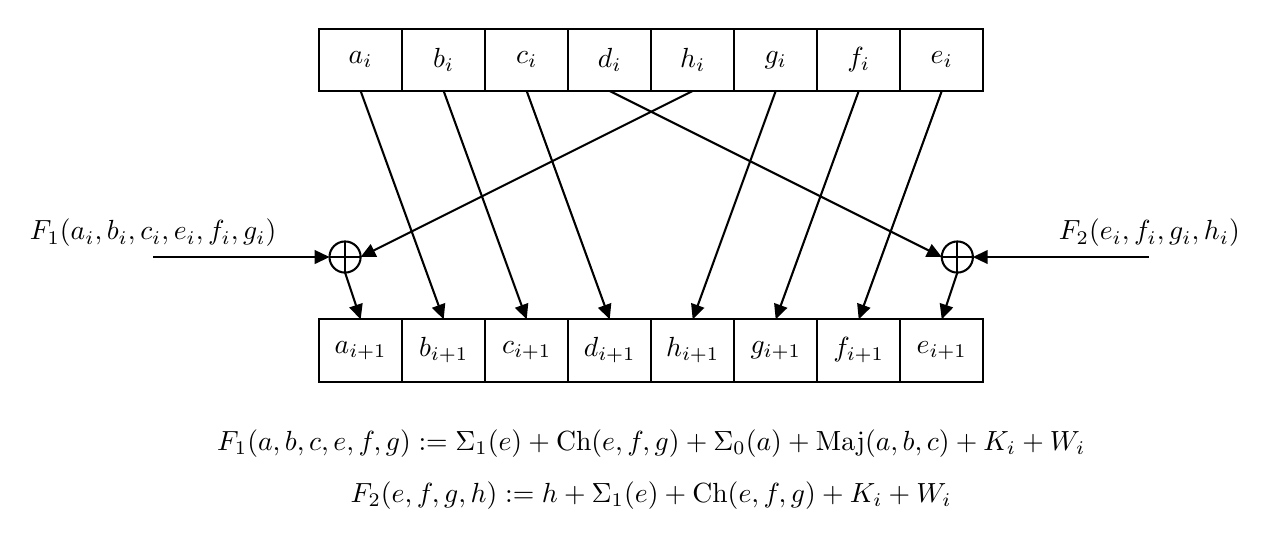
\begin{tikzpicture}[x=0.75pt,y=0.75pt,yscale=-1,xscale=1]
%uncomment if require: \path (0,253); %set diagram left start at 0, and has height of 253

%Shape: Rectangle [id:dp605201676603677] 
\draw   (100,0) -- (420,0) -- (420,30) -- (100,30) -- cycle ;
%Straight Lines [id:da7412689699456203] 
\draw    (140,0) -- (140,30) ;
%Straight Lines [id:da22647453790635086] 
\draw    (180,0) -- (180,30) ;
%Straight Lines [id:da8843056440098953] 
\draw    (220,0) -- (220,30) ;
%Straight Lines [id:da4329570184014415] 
\draw    (260,0) -- (260,30) ;
%Straight Lines [id:da4312753541741339] 
\draw    (300,0) -- (300,30) ;
%Straight Lines [id:da8624712063258593] 
\draw    (340,0) -- (340,30) ;
%Straight Lines [id:da48275098633745395] 
\draw    (380,0) -- (380,30) ;
%Shape: Rectangle [id:dp4067435943587554] 
\draw   (100,140) -- (420,140) -- (420,170) -- (100,170) -- cycle ;
%Straight Lines [id:da9101745062627391] 
\draw    (140,140) -- (140,170) ;
%Straight Lines [id:da6991884949951528] 
\draw    (180,140) -- (180,170) ;
%Straight Lines [id:da7121791754293847] 
\draw    (220,140) -- (220,170) ;
%Straight Lines [id:da006685736169755652] 
\draw    (260,140) -- (260,170) ;
%Straight Lines [id:da5006459019159044] 
\draw    (300,140) -- (300,170) ;
%Straight Lines [id:da2102106457102897] 
\draw    (340,140) -- (340,170) ;
%Straight Lines [id:da6413953387094566] 
\draw    (380,140) -- (380,170) ;
%Straight Lines [id:da9364234050345828] 
\draw    (120,30) -- (158.97,137.18) ;
\draw [shift={(160,140)}, rotate = 250.02] [fill={rgb, 255:red, 0; green, 0; blue, 0 }  ][line width=0.08]  [draw opacity=0] (7.14,-3.43) -- (0,0) -- (7.14,3.43) -- cycle    ;
%Straight Lines [id:da19670568284282752] 
\draw    (160,30) -- (198.97,137.18) ;
\draw [shift={(200,140)}, rotate = 250.02] [fill={rgb, 255:red, 0; green, 0; blue, 0 }  ][line width=0.08]  [draw opacity=0] (7.14,-3.43) -- (0,0) -- (7.14,3.43) -- cycle    ;
%Straight Lines [id:da9941673597047744] 
\draw    (200,30) -- (238.97,137.18) ;
\draw [shift={(240,140)}, rotate = 250.02] [fill={rgb, 255:red, 0; green, 0; blue, 0 }  ][line width=0.08]  [draw opacity=0] (7.14,-3.43) -- (0,0) -- (7.14,3.43) -- cycle    ;
%Straight Lines [id:da847071183150921] 
\draw    (320,30) -- (281.03,137.18) ;
\draw [shift={(280,140)}, rotate = 289.98] [fill={rgb, 255:red, 0; green, 0; blue, 0 }  ][line width=0.08]  [draw opacity=0] (7.14,-3.43) -- (0,0) -- (7.14,3.43) -- cycle    ;
%Straight Lines [id:da173533587645454] 
\draw    (360,30) -- (321.03,137.18) ;
\draw [shift={(320,140)}, rotate = 289.98] [fill={rgb, 255:red, 0; green, 0; blue, 0 }  ][line width=0.08]  [draw opacity=0] (7.14,-3.43) -- (0,0) -- (7.14,3.43) -- cycle    ;
%Straight Lines [id:da8735387545373061] 
\draw    (400,30) -- (361.03,137.18) ;
\draw [shift={(360,140)}, rotate = 289.98] [fill={rgb, 255:red, 0; green, 0; blue, 0 }  ][line width=0.08]  [draw opacity=0] (7.14,-3.43) -- (0,0) -- (7.14,3.43) -- cycle    ;
%Straight Lines [id:da32769861464522565] 
\draw    (240,30) -- (397.32,108.66) ;
\draw [shift={(400,110)}, rotate = 206.57] [fill={rgb, 255:red, 0; green, 0; blue, 0 }  ][line width=0.08]  [draw opacity=0] (7.14,-3.43) -- (0,0) -- (7.14,3.43) -- cycle    ;
%Straight Lines [id:da843529959376234] 
\draw    (280,30) -- (122.68,108.66) ;
\draw [shift={(120,110)}, rotate = 333.43] [fill={rgb, 255:red, 0; green, 0; blue, 0 }  ][line width=0.08]  [draw opacity=0] (7.14,-3.43) -- (0,0) -- (7.14,3.43) -- cycle    ;
%Flowchart: Or [id:dp6645760821949267] 
\draw   (105,110) .. controls (105,105.86) and (108.36,102.5) .. (112.5,102.5) .. controls (116.64,102.5) and (120,105.86) .. (120,110) .. controls (120,114.14) and (116.64,117.5) .. (112.5,117.5) .. controls (108.36,117.5) and (105,114.14) .. (105,110) -- cycle ; \draw   (105,110) -- (120,110) ; \draw   (112.5,102.5) -- (112.5,117.5) ;
%Straight Lines [id:da07315377917091626] 
\draw    (112.5,117.5) -- (119.05,137.15) ;
\draw [shift={(120,140)}, rotate = 251.57] [fill={rgb, 255:red, 0; green, 0; blue, 0 }  ][line width=0.08]  [draw opacity=0] (7.14,-3.43) -- (0,0) -- (7.14,3.43) -- cycle    ;
%Flowchart: Or [id:dp5992738702372278] 
\draw   (400,110) .. controls (400,105.86) and (403.36,102.5) .. (407.5,102.5) .. controls (411.64,102.5) and (415,105.86) .. (415,110) .. controls (415,114.14) and (411.64,117.5) .. (407.5,117.5) .. controls (403.36,117.5) and (400,114.14) .. (400,110) -- cycle ; \draw   (400,110) -- (415,110) ; \draw   (407.5,102.5) -- (407.5,117.5) ;
%Straight Lines [id:da3032162844879227] 
\draw    (407.5,117.5) -- (400.95,137.15) ;
\draw [shift={(400,140)}, rotate = 288.43] [fill={rgb, 255:red, 0; green, 0; blue, 0 }  ][line width=0.08]  [draw opacity=0] (7.14,-3.43) -- (0,0) -- (7.14,3.43) -- cycle    ;
%Straight Lines [id:da5583137617955998] 
\draw    (20,110) -- (102,110) ;
\draw [shift={(105,110)}, rotate = 180] [fill={rgb, 255:red, 0; green, 0; blue, 0 }  ][line width=0.08]  [draw opacity=0] (7.14,-3.43) -- (0,0) -- (7.14,3.43) -- cycle    ;
%Straight Lines [id:da3517569841519508] 
\draw    (418,110) -- (500,110) ;
\draw [shift={(415,110)}, rotate = 0] [fill={rgb, 255:red, 0; green, 0; blue, 0 }  ][line width=0.08]  [draw opacity=0] (7.14,-3.43) -- (0,0) -- (7.14,3.43) -- cycle    ;

% Text Node
\draw (20,106.6) node [anchor=south] [inner sep=0.75pt]    {$F_{1}( a_{i} ,b_{i} ,c_{i} ,e_{i} ,f_{i} ,g_{i})$};
% Text Node
\draw (500,106.6) node [anchor=south] [inner sep=0.75pt]    {$F_{2}( e_{i} ,f_{i} ,g_{i} ,h_{i})$};
% Text Node
\draw (120,15) node    {$a_{i}$};
% Text Node
\draw (160,15) node    {$b_{i}$};
% Text Node
\draw (200,15) node    {$c_{i}$};
% Text Node
\draw (240,15) node    {$d_{i}$};
% Text Node
\draw (280,15) node    {$h_{i}$};
% Text Node
\draw (320,15) node    {$g_{i}$};
% Text Node
\draw (360,15) node    {$f_{i}$};
% Text Node
\draw (400,15) node    {$e_{i}$};
% Text Node
\draw (120,155) node    {$a_{i+1}$};
% Text Node
\draw (160,155) node    {$b_{i+1}$};
% Text Node
\draw (200,155) node    {$c_{i+1}$};
% Text Node
\draw (240,155) node    {$d_{i+1}$};
% Text Node
\draw (280,155) node    {$h_{i+1}$};
% Text Node
\draw (320,155) node    {$g_{i+1}$};
% Text Node
\draw (360,155) node    {$f_{i+1}$};
% Text Node
\draw (400,155) node    {$e_{i+1}$};
% Text Node
\draw (260,200) node    {$F_{1}( a,b,c,e,f,g) :=\Sigma _{1}( e) +\mathrm{Ch}( e,f,g) +\Sigma _{0}( a) +\mathrm{Maj}( a,b,c) +K_{i} +W_{i}$};
% Text Node
\draw (260,225) node    {$F_{2}( e,f,g,h) :=h+\Sigma _{1}( e) +\mathrm{Ch}( e,f,g) +K_{i} +W_{i}$};


\end{tikzpicture}
	\caption{SHA256分组密码的一轮}
	\label{fig:8-8}
\end{figure}
 
\subsection{其他 Merkle-Damg{\aa}rd 哈希函数}\label{subsec:8-6-1}

\begin{snote}[MD4和MD5。]
这两个密码学哈希函数都是由 Ron Rivest 在1990 到 1991 年设计的。它们两者都是 Merkle-Damg{\aa}rd 哈希函数,输出 $128$ 比特的摘要。它们非常相似,尽管 MD5 使用了比 MD4 更强的压缩函数。如表 \ref{tab:8-1} 所示,已经有算法能够有效地找到这两个哈希函数的碰撞。因此,它们都不应该再被使用在现实世界的系统之中。
\end{snote}

\begin{snote}[Whirpool。]
Whirlpool 由 Barreto 和 Rijmen 在 2000 年设计,并在 2004 年被采纳为 ISO/IEC 标准。Whirpool 是一个 Merkle-Damg{\aa}rd 哈希函数。它的压缩函数使用 Miyaguchi-Preneel 方法(见图 \ref{fig:8-7})和一个名为 $W$ 的分组密码。这个分组密码与 AES 非常相似,但是分组长度为 $512$ 比特。由此产生的哈希输出也是 $512$ 比特。
\end{snote}

\begin{snote}[其他算法。]
还有一些文献提出了许多其他的 Merkle-Damg{\aa}rd 哈希函数,比如 Tiger/192 和 RIPEMD-160。
\end{snote}
\section{案例研究:HMAC}
\section{海绵构造与 SHA3}
\section{Merkle树:证明哈希列表的属性}\label{sec:8-9}
\section{密钥派生与随机预言机模型}\label{sec:8-10}

尽管像 SHA256 这样的哈希函数在起初只是为了提供抗碰撞性而被设计的,但是正如我们在 \ref{sec:8-7} 节中看到的,业界经常用它们来解决其他的一些问题。直观地说,像 SHA256 这样的哈希函数能够``彻底扰乱"其输入,因此这种方法似乎有一定的意义。事实上,在 \ref{sec:8-7} 节中,我们研究了把一个无密钥哈希函数变成一个带密钥函数的问题,后者同时也是一个安全的 PRF,我们还发现,在合理的假设下,我们确实可以给出一个安全分析。

在这一节中,我们研究另一个问题,称为\textbf{密钥派生 (key derivation)}问题。粗略的说,这个问题是这样的:我们现在有一些机密数据,并且想要把它转换成一个 $n$ 比特的序列,而后者可以作为密钥被用到其他密码学原语——比如 AES——中。现在,这种机密数据在某种意义上说可能是随机的(至少在某种程度上是难以猜测的),但它可能根本不像是一个均匀分布的、随机的、$n$ 比特的序列。那么,我们如何从这样一个秘密的 $s$ 得到一个密码学密钥 $t$ 呢? 当然是哈希。在实践中,我们需要一个哈希函数 $H$,例如 SHA256(或者,正如我们后面将要推荐的一些由 SHA256 构建的函数),并计算 $t\leftarrow H(s)$。

在介绍上述问题的同时,我们还将介绍\emph{随机预言机模型(random oracle model)},它是一个启发式工具,不仅对分析密钥派生问题有帮助,对分析其他一系列问题也是有用的。

\subsection{密钥派生问题}\label{subsec:8-10-1}

让我们更详细地考察密钥派生问题。高层次地说,该问题就是将某个难以猜测的离散数据转换为一个 $n$ 比特的序列,后者可以作为一些标准的密码学原语(比如 AES)的密钥。在所有情况下,解决方案都是对秘密进行哈希以获得密钥。我们从一些启发性的例子开始。
\begin{itemize}
	\item 秘密可能是一个口令。虽然这样的口令可能有点难猜,但直接使用它作为 AES 密钥可能是很危险的。即使口令均匀分布在一个很大的字典中(这本身已经是一个很可疑的假设了),但将它编码为一个比特序列后,编码也肯定不是均匀分布的。很可能有相当一部分的口令对应于 AES 的``弱密钥",从而使其容易受到攻击。回顾一下,AES 的设计以随机比特序列作为密钥,所以它在这样的口令上的表现完全是另一回事。
	\item 秘密可能是一台运行中的计算机上的各种类型的系统事件记录(例如各种中断的时间,如按下的按键或鼠标移动引起的中断)。同样地,身处计算机系统之外的攻击者可能很难准确预测这种日志的内容。然而,直接使用日志作为 AES 密钥是有问题的:它可能太长了,而且远不是均匀分布的。
	\item 秘密可能是一个已被部分破坏的密码学密钥。想象一下,一个用户有一个 $128$ 比特的密钥,但其中的 $64$ 比特已经被泄露给了对手。该密钥仍然相当难以猜测,但从对手的角度来看,它仍然不是均匀分布的,因此不应当再被直接用作 AES 密钥。
	\item 稍后,我们将看到在公钥密码学中被广泛使用的数论变换的例子。稍微跳跃一点,我们在后面将会看到,对于一个大的合模数 $N$,如果 $x$ 是一个随机选择的模 $N$ 数,而一个对手得到了 $y:=x^3 \bmod N$,它很难计算出 $x$。我们可以把 $x$ 看作是秘密,与前面的例子类似,我们可以把 $y$ 看作是泄露给对手的信息。即使在信息论意义上,$y$ 的值完全决定了 $x$,它仍然被广泛认为是难以计算的。因此,我们可能想把 $x$ 当作秘密数据,与前面例子中的方式完全相同。许多和之前一样的问题在这里也会出现,其中最重要的是,$x$ 通常比 AES 密钥长得多(通常有几千比特长)。
\end{itemize}

如前所述,实践中采用的解决方案是简单地使用哈希函数 $H$ 对秘密 $s$ 进行哈希以获得密钥 $t\leftarrow H(s)$。

现在,我们给出一个我们所追求的安全属性的正式定义。

我们假设,秘密 $s$ 是根据一些固定(且公开的)概率分布 $P$ 采样得到的。我们假设,任何这样的秘密数据都可以被编码为某个有限集 $\mathcal{S}$ 上的元素。此外,我们引入一个函数 $I$ 来对泄露 $s$ 的部分信息的事实进行建模,因此,一个试图猜测 $s$ 的对手能够获取侧信息 $I(s)$。

\begin{game}[猜测优势]\label{game:8-3}
令 $P$ 是一个定义在有限集 $\mathcal{S}$ 上的概率分布,$I$ 是一个定义在 $\mathcal{S}$ 上的函数。对于一个给定对手 $\mathcal{A}$,攻击游戏运行如下:
\begin{itemize}
	\item 挑战者根据 $P$ 随机选择 $s$,并将 $I(s)$ 发送给 $\mathcal{A}$。
	\item 对手输出对 $s$ 的猜测 $\hat{s}$,如果 $\hat{s}=s$,它就赢得该游戏。
\end{itemize}
我们称 $\mathcal{A}$ 赢得该游戏的概率为其\textbf{猜测优势(guessing advantage)},记为 $\mathrm{Guess}\mathsf{adv}[\mathcal{A},P,I]$。
\end{game}

在上面的第一个例子中,我们可以简单地将 $s$ 建模为一个口令,这个口令均匀分布在某个(已被编码的)字典 $D$ 上。在这种情况下,对手没有得到任何侧信息,不管它的算力有多强,猜测优势都是 $1/|D|$。

在上面的第二个例子中,我们似乎很难对猜测优势给出一个有意义的、可靠的估计。

在上面的第三个例子中,$s$ 均匀分布在 $\{0,1\}^{128}$ 上,而 $I(s)$ 是 $s$ 的前 $64$ 比特。显然,任何对手,无论其算力多么强大,猜测优势都不会超过 $2^{-64}$。

在上面的第四个例子中,$s$ 是值 $x$,$I(s)$ 是值 $y$。由于 $y$ 完全决定了 $x$,所以对手有可能通过暴力搜索由 $I(s)$ 恢复 $s$。当然也有更聪明和更快的算法,但目前还没有已知的有效算法可以做到这一点。所以对于所有有效对手,猜测优势似乎都是可忽略不计的。

现在,假设我们使用一个哈希函数 $H:\mathcal{S}\to\mathcal{T}$ 从 $s$ 派生出密钥 $t$。直观地说,我们想让 $t$ ``看起来是随机的"。为了正式地定义这个直观的概念,我们使用 \ref{sec:3-11} 节中定义的计算上不可区分性的概念。因此,正式地说,我们想要的属性是:如果 $s$ 是根据 $P$ 采样得到的,而 $t$ 是从 $\mathcal{T}$ 中随机选出的,那么两个分布 $(I(s),H(s))$ 和 $(I(s),t)$ 在计算上是不可区分的。对于对手 $\mathcal{A}$,令 $\mathrm{Dist}\mathsf{adv}[\mathcal{A},P,I,H]$ 是对手在攻击游戏 \ref{game:3-3} 中区分这两种分布的优势。

对于我们希望能够证明的定理,它的类型是,大体上说,如果 $H$ 满足某个特定属性,或许 $P$ 和 $I$ 也被施加了某种约束,那么对于每个对手 $\mathcal{A}$,都存在一个对手 $\mathcal{B}$(它是一个 $\mathcal{A}$ 的基本包装器),满足 $\mathrm{Dist}\mathsf{adv}[\mathcal{A},P,I,H]$ 不比 $\mathrm{Guess}\mathsf{adv}[\mathcal{B},P,I]$ 大太多。事实上,在某些情况下,证明这样一个定理\emph{是}可能的。我们将在后面的 \ref{subsec:8-10-4} 小节中讨论这个结论——现在,我们简单地说,由于一些原因,这种严格的方法在实践中并没有被广泛地使用。相反,我们将更详细地研究使用 SHA256 这样``现成"的哈希函数来派生密钥的启发式方法。

\begin{snote}[子密钥的派生。]
在继续我们的讨论之前,我们考虑以下相关的问题:如何处理从 $s$ 派生来的密钥 $t$。在某些应用中,我们可能会直接使用 $t$ 作为——比方说——AES 的密钥。然而,在其他应用中,我们可能需要好几个密钥:例如一个加密密钥和一个 MAC 密钥,或者用于安全双工通信的两个不同的加密密钥(因此,Alice 有一个密钥用于向 Bob 发送加密消息,而 Bob 使用另一个密钥向 Alice 发送加密消息)。因此,一旦我们派生出一个``就所有意图和目的而言"都表现得像一个随机比特序列的单一密钥 $t$,我们就想再派生出几个子密钥。我们称之为\textbf{子密钥派生问题(sub-key derivation problem)},以区别于密钥派生问题。对于子密钥派生问题,我们假设从一个真随机的密钥 $t$ 开始,但是 $t$ 很可能并不是真随机的,但是当 $t$ 与真随机的密钥在计算上不可区分时,这个假设就是合理的。

幸运的是,对于子密钥派生问题,我们已经掌握了我们所需的所有工具。事实上,我们可以使用 PRG 或 PRF 从 $t$ 派生出子密钥。例如,在上面的例子中,如果 Alice 和 Bob 已经有了一个共享密钥 $t$,而它是由一个秘密 $s$ 派生而来的,那么他们就可以按如下方式使用 PRF $F$:
\begin{itemize}
	\item 派生出一个 MAC 密钥 $k_\mathrm{mac}\overset{\rm R}\leftarrow F(t,\,\texttt{"MAC}\text{-}\texttt{KEY"})$。
	\item 派生出一个 Alice 到 Bob 的加密密钥 $k_\mathrm{AB}\overset{\rm R}\leftarrow F(t,\texttt{"AB}\text{-}\texttt{KEY"})$。
	\item 派生出一个 Bob 到 Alice 的加密密钥 $k_\mathrm{BA}\overset{\rm R}\leftarrow F(t,\texttt{"BA}\text{-}\texttt{KEY"})$。
\end{itemize}
假设 $F$ 是一个安全的 PRF,那么密钥 $k_\mathrm{mac}$、$k_\mathrm{AB}$ 和 $k_\mathrm{BA}$ 的行为,就所有意图和目的而言,都像是独立的随机密钥。为了实现 $F$,我们甚至可以使用基于哈希的 PRF(如 HMAC),所以我们可以使用单一的``现成"哈希函数,如 SHA256,来完成我们所需要的一切任务,即密钥派生和子密钥派生。

因此,一旦我们解决了密钥派生的问题,我们就可以使用所构建的工具来解决子密钥派生的问题。不幸的是,使用``现成"的哈希函数进行密钥派生的做法并没有得到很好的理解和分析。尽管如此,还是有一些有用的启发式模型可供探索。
\end{snote}

\subsection{随机预言机:一种有用的启发法}\label{subsec:8-10-2}

我们现在介绍一种启发式算法,它可以在各种应用中被用来模拟哈希函数,包括密钥派生。正如我们将要在后面的章节中看到的,它已经成为一种流行的启发式算法,被用来证明许多密码学构造的合理性。

我们的想法是,简单地对哈希函数 $H$ 进行建模,\emph{就好像}它是一个真随机函数 $\mathcal{O}$ 一样。如果 $H$ 将 $\mathcal{M}$ 映射成 $\mathcal{T}$,那么 $\mathcal{O}$ 就是从集合 $\mathrm{Funs}[\mathcal{M},\mathcal{T}]$ 中均匀随机选出的。我们可以将任何攻击游戏转化为它的随机预言机版本:挑战者用 $\mathcal{O}$ 代替 $H$ 进行所有的计算,此外,对手被允许在它所选定的任意输入点上查询并获取 $\mathcal{O}$ 的值。这个函数 $\mathcal{O}$ 被称为\textbf{随机预言机 (random oracle)}。在这种设定下,我们称安全性在\textbf{随机预言机模型 (random oracle model)}下成立。由于函数 $\mathcal{O}$ 实在太大,我们无法将它写下来,更不可能将它用在真正的构造中。相对地,只有在对实际使用 $H$ 的系统进行启发式的安全分析时,我们才会用到 $\mathcal{O}$。

这种对使用哈希函数的构造进行分析的方法类似于 \ref{sec:4-7} 节所介绍的\emph{理想密码模型}。回顾一下,在理想密码模型中,我们用一个随机置换族 $\{\Pi_\mathpzc{k}\}_{\mathpzc{k}\in\mathcal{K}}$ 来替代一个定义在 $(\mathcal{K},\mathcal{X})$ 上的分组密码 $\mathcal{E}=(E,D)$。

正如我们之前所说的,随机预言机模型在现代密码学中用得很多。如果我们能使用一个``现成"的哈希函数 $H$,并将其建模为一个随机预言机,那就更好了。然而,如果我们想要一个真正通用的工具,我们就必须得小心一点,特别是如果我们想把 $H$ 建模为一个接受\emph{变长输入}的随机预言机的话。基本的经验法则是,不要\emph{直接}将 Merkle-Damg{\aa}rd 哈希用作通用的随机预言机。我们将在 \ref{subsec:8-10-3} 小节中讨论如何安全地(但同样也是启发式地)将 Merkle-Damg{\aa}rd 哈希用作通用的随机语言机。此外,我们还将看到,海绵构造(见 \ref{sec:8-8} 节)可以直接被``原样"使用。

我们强调,即使随机预言机上的安全结论都是严格的数学定理,它们仍然只是启发式的结果,而不能为使用特定哈希函数构建的系统提供任何安全性保证。尽管如此,这些安全结论确实能够排除针对系统的``通用攻击",如果哈希函数\emph{是}一个随机预言机的话,后者确实\emph{是}可行的。因此,这样的结论虽然不能排除所有攻击,但确实能够排除一般的攻击,这显然比对系统的安全性完全没有任何说法要好得多。事实上,在现实世界中,如果需要在两个系统 $\mathcal{S}_1$ 和 $\mathcal{S}_2$ 之间做一个选择,其中 $\mathcal{S}_1$ 有一个在随机预言机模型下的安全证明,而 $\mathcal{S}_2$ 有一个真正的安全证明,但是它的运行时间却是 $\mathcal{S}_1$ 的两倍,那么大多数业者都会(非常合理地)选择 $\mathcal{S}_1$,而不是 $\mathcal{S}_2$。

\begin{snote}[在随机预言机模型下定义安全性。]
假设我们有某种类型的密码学方案 $\mathcal{S}$,其实现使用了一个子程序,用于计算一个定义在 $(\mathcal{M},\mathcal{T})$ 上的哈希函数 $H$。方案 $\mathcal{S}$ 在其选择的任意点上评估 $H$,但不会考察 $H$ 的内部实现。我们称 \textbf{$\mathcal{S}$ 将 $H$ 用作一个预言机 ($\mathcal{S}$ uses $H$ as an oracle)}。比如说我们曾在 \ref{sec:8-7} 节中简要考察的方案 $F_\mathrm{pre}(k,x):=H(k\,\Vert\,x)$,它就是一个将哈希函数 $H$ 用作预言机的 PRF。

我们想要分析 $\mathcal{S}$ 的安全性。我们假设我们所感兴趣的任何安全属性,比如说一个``属性 $X$",(像往常一样)被建模为挑战者(特定于属性 $X$)和一个任意的对手 $\mathcal{A}$ 之间的游戏。在应答特定查询时,挑战者想必会计算与方案 $\mathcal{S}$ 相关的各种函数,而这些函数又可能需要在某些点上对 $H$ 进行评估。这个游戏定义了一个优势 $\mathrm{X}\mathsf{adv}[\mathcal{A},\mathcal{S}]$,而关于属性 $X$ 的安全性意味着,对于所有有效对手 $\mathcal{A}$,该优势都应当是可忽略不计的。

如果我们想要在随机预言机模型下分析 $\mathcal{S}$,定义安全性的攻击游戏就需要被修改,使用一个\emph{真随机函数} $\mathcal{O}\in\mathrm{Funs}[\mathcal{M},\mathcal{T}]$ 有效地替代 $H$,而对手和挑战者都可以对后者发起预言机访问。更确切地说,该游戏应当被修改如下:
\begin{itemize}
	\item 在游戏开始时,挑战者随机选择一个 $\mathcal{O}\in\mathrm{Funs}[\mathcal{M},\mathcal{T}]$。
	\item 除了标准查询外,对手 $\mathcal{A}$ 还可以提交\emph{随机预言机查询 (random oracle queries)}:它向挑战者发送 $m\in\mathcal{M}$,而挑战者用 $t=\mathcal{O}(m)$ 应答。对手可以发起任意数量的随机预言机查询,并且可以与标准查询以任意次序交错进行。
	\item 在处理标准查询时,挑战者用 $\mathcal{O}$ 来代替 $H$ 来进行计算。
\end{itemize}
定义对手优势的规则与之前相同,但使用 $\mathrm{X}^\mathrm{io}\mathsf{adv}[\mathcal{A},\mathcal{S}]$ 来表示,以强调这是随机预言机模型下的优势。\emph{随机预言机模型下}的安全性意味着,对于所有有效对手 $\mathcal{A}$,$\mathrm{X}^\mathrm{io}\mathsf{adv}[\mathcal{A},\mathcal{S}]$ 都是可忽略不计的。
\end{snote}

\begin{snote}[一个简单的例子:随机预言机模型下的 PRF。]
下面,我们说明如何应用随机预言机框架来构建安全的 PRF。特别地,我们将表明,在随机预言机模型下,$F_\mathrm{pre}$ 是一个安全的 PRF。我们首先修改标准的 PRF 安全游戏,以获得随机预言机模型下的 PRF 安全游戏。为了更清楚地表述问题,如果我们有一个将哈希函数 $H$ 用作预言机的 PRF,我们就用 $F^\mathcal{O}$ 表示使用随机预言机 $\mathcal{O}$ 代替 $H$ 后得到的函数。
\end{snote}

\begin{game}[随机预言机模型下的 PRF]\label{game:8-4}
令 $F$ 是一个定义在 $(\mathcal{K},\mathcal{X},\mathcal{Y})$ 上的 PRF,它将一个定义在 $(\mathcal{M},\mathcal{T})$ 上的哈希函数 $H$ 用作预言机。对于一个给定对手 $\mathcal{A}$,我们定义两个实验:实验 $0$ 和实验 $1$。对于 $b=0,1$,我们定义:

\noindent\textbf{实验 $b$:}
\begin{itemize}
	\item 挑战者按如下方式选择 $f\in{\rm Funs}[\mathcal{X},\mathcal{Y}]$:
	
	\hspace*{26pt} 如果 $b=0$:随机选取 $k\overset{\rm R}\leftarrow\mathcal{K}$,令 $f\leftarrow F^\mathcal{O}(k,\cdot)$;\\
	\hspace*{26pt} 如果 $b=1$:随机选取 $f\overset{\rm R}\leftarrow{\rm Funs}[\mathcal{X},\mathcal{Y}]$。
	
	\item 对手向挑战者发起一系列查询。
	\begin{itemize}
		\item $F$-查询:对于查询 $x\in\mathcal{X}$,应答 $y=f(x)\in\mathcal{Y}$。
		\item $\mathcal{O}$-查询:对于查询 $m\in\mathcal{M}$,应答 $t=\mathcal{O}(m)\in\mathcal{T}$。
	\end{itemize}
	\item 对手计算并输出一个比特 $\hat b\in\{0,1\}$。
\end{itemize}
对于 $b=0,1$,令 $W_b$ 为 $\mathcal{A}$ 在实验 $b$ 中输出 $1$ 的事件。我们将 $\mathcal{A}$ 就 $F$ 的优势定义为:
\[
\mathrm{PRF}^\mathrm{ro}\mathsf{adv}[\mathcal{A},F]:=
\big\lvert
\Pr[W_0]-\Pr[W_1]
\big\rvert
\]
\end{game}

\begin{definition}\label{def:8-5}
如果对于所有有效对手 $\mathcal{A}$,$\mathrm{PRF}^\mathrm{ro}\mathsf{adv}[\mathcal{A},F]$ 的值都是可忽略不计的,我们就称 PRF $F$ 在随机预言机模型下是安全的。
\end{definition}

重新考虑 PRF $F_\mathrm{pre}(k,x):=H(k\,\Vert\,x)$。我们假设 $F_\mathrm{pre}$ 定义在 $(\mathcal{K},\mathcal{X},\mathcal{T})$ 上,其中 $\mathcal{K}=\{0,1\}^\kappa$,$\mathcal{X}=\{0,1\}^{\leq L}$,并且 $H$ 定义在 $(\mathcal{M},\mathcal{T})$ 上,其中 $\mathcal{M}$ 包括所有最长为 $\kappa+L$ 的比特序列。

我们将证明,在随机预言机模型下,该 PRF 是一个安全的 PRF。但是等等!我们已经在 \ref{sec:8-7} 节中论证过,当 $H$ 是一个 Merkle-Damg{\aa}rd 哈希时,$F_\mathrm{pre}$ 完全是不安全的。这似乎出现了矛盾。问题在于,正如我们之前提到的,直接使用 Merkle-Damg{\aa}rd 哈希作为随机预言机是不安全的。我们将在 \ref{subsec:8-10-3} 节介绍解决这个问题的方法。

\begin{theorem}\label{theo:8-9}
如果 $\mathcal{K}$ 很大,那么当 $H$ 被建模为一个随机预言机时,$F_\mathrm{pre}$ 就是一个安全的 PRF。
\begin{quote}
特别地,如果 $\mathcal{A}$ 是一个如攻击游戏 \ref{game:8-4} 中那样的随机预言机 PRF 对手,并且最多可以发起 $Q_\mathrm{ro}$ 次预言机查询,则有:
\end{quote}
\[
\mathrm{PRF}^\mathrm{ro}\mathsf{adv}[\mathcal{A},F_\mathrm{pre}]
\leq
Q_\mathrm{ro}/|\mathcal{K}|
\]
\end{theorem}

请注意,定理 \ref{theo:8-9} 是无条件成立的,也就是说,对 $\mathcal{A}$ 的唯一约束就是随即预言机查询次数的限制:它不依赖于任何复杂性假设。

\begin{proof}[证明思路]
一旦将 $H$ 替换成 $\mathcal{O}$,对手就必须在不持有密钥 $k$ 的情况下将 $\mathcal{O}(k\,\Vert\,\cdot)$ 和 $\mathrm{Funs}[\mathcal{X},\mathcal{T}]$ 中的一个随机函数区分开来。由于 $\mathcal{O}(k\,\Vert\,\cdot)$ 也是 $\mathrm{Funs}[\mathcal{X},\mathcal{T}]$ 上的一个随机函数,因此对手唯一的希望,就是发起对 $\mathcal{O}$ 的查询,并且以某种方式利用应答所透露的信息。如果 $k'=k$,我们就称 $\mathcal{O}$-查询 $k'\,\Vert\,x'$ 是相关的。很显然,如果一个对 $\mathcal{O}$ 的查询不是相关的,它对于区分 $\mathcal{O}(k\,\Vert\,\cdot)$ 和随机函数就不会提供帮助,因为这时查询所返回的值与函数 $\mathcal{O}(k\,\Vert\,\cdot)$ 是无关的。此外,经过 $Q_\mathrm{ro}$ 次查询后,对手成功发起一次相关查询的概率最大是 $Q_\mathrm{ro}/|\mathcal{K}|$。
\end{proof}

\begin{proof}
为了严格表述上述证明思路,我们令 $\mathcal{A}$ 与两个 PRF 挑战者交互。对于 $j=0,1$,令 $W_j$ 表示 $\mathcal{A}$ 在游戏 $j$ 中输出 $1$ 的事件。

\vspace{5pt}

\noindent\textbf{游戏 $\mathbf{0}$。}
我们将游戏 $0$ 中的挑战者按如下方式表述,使得它等价于攻击游戏 \ref{game:8-4} 中的实验 $0$,但是更加便于分析。我们假设对手不会发起两次相同的 $F_\mathrm{pre}$-查询。此外,利用我们以经使用过很多次的``忠实的侏儒"的思路,我们使用一个关联数组 $Map:\mathcal{M}\to\mathcal{T}$ 来建立临时的随机预言机。下面是挑战者的运行逻辑:

\vspace{5pt}

\hspace*{5pt} 初始化:\\
\hspace*{50pt} 初始化一个空的关联数组 $Map:\mathcal{M}\to\mathcal{T}$\\
\hspace*{50pt} 随机选取 $k\overset{\rm R}\leftarrow\mathcal{K}$\\
\hspace*{26pt} 当收到一个对 $x\in\{0,1\}^{\leq L}$ 的 $F_\mathrm{pre}$-查询时:\\
\hspace*{50pt} 随机选取 $t\overset{\rm R}\leftarrow\mathcal{T}$\\
\hspace*{5pt} ($1$)
\hspace*{24.5pt} 如果 $(k\,\Vert\,x)\in\mathrm{Domain}(Map)$,就令 $t\leftarrow Map[k\,\Vert\,x]$\\
\hspace*{5pt} ($2$)
\hspace*{24.5pt} 令 $Map[k\,\Vert\,x]\leftarrow t$\\
\hspace*{50pt} 将 $t$ 发送给 $\mathcal{A}$\\
\hspace*{26pt} 当收到一个 $\mathcal{O}$-查询 $m\in\mathcal{M}$ 时:\\
\hspace*{50pt} 随机选取 $t\overset{\rm R}\leftarrow\mathcal{T}$\\
\hspace*{50pt} 如果 $m\in\mathrm{Domain}(Map)$,就令 $t\leftarrow Map[m]$\\
\hspace*{50pt} 令 $Map[m]\leftarrow t$\\
\hspace*{50pt} 将 $t$ 发送给 $\mathcal{A}$

\vspace{5pt}

\noindent
很显然,该挑战者就等价于攻击游戏 \ref{game:8-4} 的实验 $0$ 中的挑战者。在游戏 $0$ 中,每当挑战者(在处理 $F_\mathrm{pre}$-查询或 $\mathcal{O}$-查询时)需要在某个输入位置对随机预言机进行采样,它都会生成一个随机的``默认输出"。如果它发现预言机曾经在该输入位置被采样过,就会覆盖这个默认输出;在任何情况下,关联数组都会记录输入/输出对。

\vspace{5pt}

\noindent\textbf{游戏 $\mathbf{1}$。}
我们让我们的侏儒变得``健忘",方法是修改游戏 $0$,删除标有 ($1$) 和 ($2$) 的两行。现在观察一下,在游戏 $1$ 中,挑战者在应答 $F_\mathrm{pre}$-查询时,不会再使用 $Map$ 或 $k$:它只会返回一个随机值。所以很明显(根据假设,$\mathcal{A}$ 不会发起两次相同的 $F_\mathrm{pre}$-查询),游戏 $1$ 就等同于攻击游戏 \ref{game:8-4} 的实验 $1$,因此有:
\[
\mathrm{PRF}^\mathrm{ro}\mathsf{adv}[\mathcal{A},F_\mathrm{pre}]=
\big\lvert
\Pr[W_1]-\Pr[W_0]
\big\rvert
\]
令 $Z$ 为对手\emph{在游戏 $1$ 中}对一个点 $m=(k\,\Vert\,\hat{x})$ 发起 $\mathcal{O}$-查询的事件。很明显,除非 $Z$ 发生,否则上述两个游戏的结果是一样的。所以,根据差分引理,我们有:
\[
\big\lvert
\Pr[W_1]-\Pr[W_0]
\big\rvert
\leq\Pr[Z]
\]
由于密钥 $k$ 完全独立于 $\mathcal{A}$ 在游戏 $1$ 中的观察,因此每个 $\mathcal{O}$-查询都会以 $1/|\mathcal{K}|$ 的概率命中该密钥,此外,简单应用联合约束,我们就可以得到:
\[
\Pr[Z]\leq
Q_\mathrm{ro}/|\mathcal{K}|
\]
这就完成了证明。
\end{proof}

\begin{snote}[随机预言机模型下的密钥派生。]
现在,我们回到 \ref{subsec:8-10-1} 小节中讨论的密钥派生问题。同样地,我们有一个采样自某个分布 $P$ 的秘密 $s$,而信息 $I(s)$ 被泄露给了对手。我们要论证的是,如果 $H$ 被建模为一个随机预言机,那么对手在区分 $(I(s),H(s))$ 和 $(I(s),t)$(其中 $t$ 是真随机的)上的优势,不会比对手只用 $I(s)$(而不是 $H(s)$)猜出秘密 $s$ 的优势多太多。

为了将 $H$ 建模为一个随机预言机 $\mathcal{O}$,我们将计算性不可区分性攻击游戏 \ref{game:3-3} 转换为随即预言机模型,所以现在,攻击者被给予对随即预言机 $\mathcal{O}$ 的访问,并试图区分 $(I(s),\mathcal{O}(s))$ 和 $(I(s),t)$。与该攻击相关的优势被记为 $\mathrm{Dist}^\mathrm{ro}\mathsf{adv}[\mathcal{A},P,I,H]$。

在陈述我们的安全定理之前,我们不妨先对攻击游戏 \ref{game:8-3} 进行推广,允许对手输出一个猜测列表 $\hat{s}_1,\dots,\hat{s}_Q$。如果对于某个 $i=1,\dots,Q$,有 $\hat{s}_i=s$ 成立,我们就称对手赢得游戏。对手 $\mathcal{A}$ 在这个游戏中获胜的概率被称为他的\textbf{列表猜测优势(list guessing advantage)},记为 $\mathrm{ListGuess}\mathsf{adv}[\mathcal{A},P,I]$。

显然,如果一个对手 $\mathcal{A}$ 能以概率 $\epsilon$ 赢得上述列表猜测游戏,我们就可以将它转换成一个以概率 $\epsilon/Q$ 赢得单次猜测游戏的对手:我们只需运行 $\mathcal{A}$ 并得到一个列表 $\hat{s}_1,\dots,\hat{s}_Q$,然后随机选择一个 $i=1,\dots,Q$,最后输出 $\hat{s}_i$。然而有时,我们说不定能做得更好:使用部分信息 $I(s)$,我们也许就能排除一些 $\hat{s}_i$;而且,在某些情况下,我们可能能够唯一确定正确的 $\hat{s}_i$。这取决于具体的应用。
\end{snote}

\begin{theorem}\label{theo:8-10}
如果 $H$ 被建模为一个随机预言机,那么对于每个最多发起 $Q_\mathrm{ro}$ 次随机预言机查询的区分对手 $\mathcal{A}$,都存在一个列表猜测对手 $\mathcal{B}$,它是一个围绕 $\mathcal{A}$ 的基本包装器,满足:
\[
\mathrm{Dist}^\mathrm{ro}\mathsf{adv}[\mathcal{A},P,I,H]
\leq
\mathrm{ListGuess}\mathsf{adv}[\mathcal{B},P,I]
\]
并且,$\mathcal{B}$ 所输出的列表最多有 $Q_\mathrm{ro}$ 项。特别地,存在一个猜测对手 $\mathcal{B}'$,它是一个围绕 $\mathcal{A}$ 的基本包装器,满足:
\[
\mathrm{Dist}^\mathrm{ro}\mathsf{adv}[\mathcal{A},P,I,H]
\leq
Q_\mathrm{ro}\cdot\mathrm{Guess}\mathsf{adv}[\mathcal{B}',P,I]
\]
\end{theorem}

\begin{proof}
该证明与定理 \ref{theo:8-9} 的证明几乎完全相同。我们定义两个游戏,对于 $j=0,1$,令 $W_j$ 表示 $\mathcal{A}$ 在游戏 $j$ 中输出 $1$ 的事件。

\vspace{5pt}

\noindent\textbf{游戏 $\mathbf{0}$。}
我们将游戏 $0$ 中的挑战者按如下方式表述,使得它等价于 $(I(s),H(s))$ 和 $(I(s),t)$ 区分游戏的实验 $0$。我们使用一个关联数组 $Map:\mathcal{M}\to\mathcal{T}$ 来建立临时的随机预言机。下面是挑战者的运行逻辑:

\vspace{5pt}

\hspace*{5pt} 初始化:\\
\hspace*{50pt} 初始化一个空的关联数组 $Map:\mathcal{M}\to\mathcal{T}$\\
\hspace*{50pt} 根据分布 $P$ 生成 $s$\\
\hspace*{50pt} 随机选取 $t\overset{\rm R}\leftarrow\mathcal{T}$\\
\hspace*{5pt} ($*$)
\hspace*{24.5pt} 令 $Map[s]\leftarrow t$\\
\hspace*{50pt} 将 $(I(s),t)$ 发送给 $\mathcal{A}$\\
\hspace*{26pt} 当收到一个 $\mathcal{O}$-查询 $\hat{s}\in\mathcal{S}$ 时:\\
\hspace*{50pt} 随机选取 $\hat{t}\overset{\rm R}\leftarrow\mathcal{T}$\\
\hspace*{50pt} 如果 $\hat{s}\in\mathrm{Domain}(Map)$,就令 $\hat{t}\leftarrow Map[\hat{s}]$\\
\hspace*{50pt} 令 $Map[\hat{s}]\leftarrow\hat{t}$\\
\hspace*{50pt} 将 $\hat{t}$ 发送给 $\mathcal{A}$

\vspace{5pt}

\noindent\textbf{游戏 $\mathbf{1}$。}
我们删除标有 ($*$) 的那一行。该游戏就等同于区分游戏的实验 $1$,因为现在的 $t$ 值是真正独立于随机预言机的。此外,除非游戏 $1$ 中的对手 $\mathcal{A}$ 在 $s$ 处发起了一个 $\mathcal{O}$-查询,否则这两个游戏的结果就是一样的。所以,我们的列表猜测对手 $\mathcal{B}$ 只是从自己的挑战者那里得到值 $I(s)$,并像游戏 $1$ 中那样扮演 $\mathcal{A}$ 的挑战者的角色。在游戏结束时,$\mathcal{B}$ 简单地输出 $\mathrm{Domain}(Map)$,即 $\mathcal{A}$ 发起的所有 $\mathcal{O}$-查询的位置。重要的一点是:我们的 $\mathcal{B}$ 在扮演这个角色时,除了 $I(s)$ 之外,没有获得任何其他关于 $s$ 的信息,此外,它记录了 $\mathcal{A}$ 所发起的所有 $\mathcal{O}$-查询。所以,根据查分引理,我们有:
\[
\mathrm{Dist}^\mathrm{ro}\mathsf{adv}[\mathcal{A}]=
\big\lvert
\Pr[W_0]-\Pr[W_1]
\big\rvert
\leq
\mathrm{ListGuess}\mathsf{adv}[\mathcal{B}]\qedhere
\]
\end{proof}

\subsection{随机预言机:安全的操作模式}\label{subsec:8-10-3}

我们已经看到,在随机预言机模型下,$F_\mathrm{pre}(k,x):=H(k\,\Vert\,x)$ 是安全的。然而,我们还知道,如果 $H$ 是一个 Merkle-Damg{\aa}rd 哈希,它就完全是不安全的。问题在于,Merkle-Damg{\aa}rd 构造包含一个非常简单的迭代结构,这将它暴露在``扩展攻击"之下。虽然从抗碰撞的角度来看,这种构造并不是问题,但它表明,拿一个现成的哈希函数并把它当作一个随机预言机来使用是一个非常危险的举措。

在本节中,我们将讨论如何安全地将一个 Merkle-Damg{\aa}rd 哈希函数用作一个随机预言机。我们还将看到,海绵构造(见 \ref{sec:8-8} 节)已经可以安全地``按原样"使用;事实上,海绵构造正是为该目的设计的:提供一个可以直接被用作随机预言机的,针对变长输入和变长输出的哈希函数。

假设 $H$ 是一个由压缩函数 $h:\{0,1\}^n\times\{0,1\}^\ell\to\{0,1\}^n$ 构建的 Merkle-Damg{\aa}rd 哈希。一个推荐的操作模式是使用 HMAC 和零密钥:
\[
\mathrm{HMAC}_0(m)
:=\mathrm{HMAC}(0^\ell,m)
=H\big(\mathsf{opad}\,\Vert\,H(\mathsf{ipad}\,\Vert\,m)\big)
\]
虽然这个构造能够挫败明显的扩展攻击,但我们凭什么相信 $\mathrm{HMAC}_0$ 作为一个通用的随机预言机是安全的?事实上,我们只能给出启发式的证据。从本质上讲,我们想要论证的是,$\mathrm{HMAC}_0$ 不存在内生的结构性弱点,它能招致将底层压缩函数本身作为随机预言机的通用攻击——或者,更现实地说——将底层压缩函数作为一个基于理想密码的 Davies-Meyer 构造的通用攻击。

因此我们想表明,利用某些特定的操作模式,我们可以由一个``小"的随机预言机,一个理想密码,甚至一个理想置换,建立一个``大"的随机预言机。

用来完成这种任务的数学工具被称为\textbf{无差别性(indifferentiability)}。我们在这里介绍此概念的一个简化版本。假设我们试图由一个较小的原语 $\rho$ 建立一个``大"的随机预言机 $\mathcal{O}$,其中 $\rho$ 可以是一个小领域上的随机预言机,一个理想密码,或者一个理想置换。我们用 $F[\rho]$ 表示基于理想原语 $\rho$ 的随机预言机的一个特定构造。

现在,考虑由某个挑战者 $\mathbf{C}$ 和对手 $\mathcal{A}$ 定义的一个通用攻击游戏。我们将 $\mathbf{C}$ 和 $\mathcal{A}$ 之间的交互记为 $\langle\mathbf{C},\mathcal{A}\rangle$。我们假设交互的结果是一个输出比特。我们接下来的所有安全定义都以这种形式的游戏为模型。

在有大随机预言机 $\mathcal{O}$ 的攻击游戏的随机预言机版本中,我们会允许挑战者和对手对随机函数 $\mathcal{O}$ 发起预言机访问,我们将交互记为 $\langle\mathbf{C}^\mathcal{O},\mathcal{A}^\mathcal{O}\rangle$。然而,如果我们使用构造 $F[\rho]$ 来实现上述的大随机预言机,那么,尽管挑战者只会通过构造 $F$ 来访问 $\rho$,对手却能够直接查询 $\rho$。我们将这种交互记为 $\langle\mathbf{C}^{F[\rho]},\mathcal{A}^\rho\rangle$。

例如,在 $\mathrm{HMAC}_0$ 构造中,压缩函数 $h$ 被建模为一个随机预言机 $\rho$;或者,如果 $h$ 本身是通过 Davies-Meyer 构建的,那么底层的分组密码就被建模为一个理想密码 $\rho$。 在任何一种情况下,$F[\rho]$ 都对应于 $\mathrm{HMAC}_0$ 构造本身。请注意,这里存在一种不对称性:在任何攻击游戏中,挑战者都只能通过 $F[\rho]$(本例中为 $\mathrm{HMAC}_0$)间接地访问 $\rho$,而对手却可以直接访问 $\rho$ 本身(即压缩函数 $h$ 或底层的分组密码)。

如果以下结论成立,我们就称 $F[\rho]$ 与 $\mathcal{O}$ 是\textbf{无差别(indifferentiable)}的:
\begin{quote}
\emph{对于每个有效挑战者 $\mathbf{C}$ 和有效对手 $\mathcal{A}$,都存在一个有效对手 $\mathcal{B}$,它是一个围绕 $\mathcal{A}$ 的基本包装器,满足:}
\end{quote}
\[
\big\lvert
\Pr[\langle\mathbf{C}^{F[\rho]},\mathcal{A}^\rho\rangle \text{ output } 1]
-
\Pr[\langle\mathbf{C}^\mathcal{O},\mathcal{B}^\mathcal{O}\rangle  \text{ output } 1]
\big\rvert
\]
\begin{quote}
\emph{是可忽略不计的。}
\end{quote}

从定义中应该可以看出,如果我们能够在随机预言机模型下为大的随机预言机 $\mathcal{O}$ 证明某个密码学方案的安全性,那么如果我们用 $F[\rho]$ 来实现 $\mathcal{O}$,该方案就仍然是安全的:如果一个对手 $\mathcal{A}$ 能够攻破使用 $F[\rho]$ 的方案,那么上面的对手 $\mathcal{B}$ 就能够攻破使用 $\mathcal{O}$ 的方案。

\begin{snote}[一些安全的模式。]
如果我们将压缩函数 $h$ 本身建模为一个随机预言机,或者 $h$ 是通过 Davies-Meyer 构建的,并且我们将底层分组密码建模为一个理想密码,我们就可以证明 $\mathrm{HMAC}_0$ 构造与变长输入上的随机预言机是无差别的。

将 $\mathrm{HMAC}_0$ 直接用作随机预言机的一个问题是,它的\emph{输出}相当短。幸运的是,使用 $\mathrm{HMAC}_0$ 来获得一个具有较长输出的随机预言机其实并不困难。方法如下。假设 $\mathrm{HMAC}_0$ 的输出有 $n$ 比特,而我们需要一个长输出(比如说 $N>n$ 比特)的随机预言机。设置 $q:=\lceil N/n\rceil$。令 $e_0,e_1,\dots,e_q$ 是整数 $0,1,\dots,q$ 的定长编码。我们的新哈希函数 $H'$ 按如下方式工作。对于输入 $m$,我们计算 $t\leftarrow\mathrm{HMAC}_0(e_0\,\Vert\,m)$。然后,对于 $i=1,\dots,q$,我们计算 $t\leftarrow\mathrm{HMAC}_0(e_i\,\Vert\,t)$。最后,我们输出 $t_1\,\Vert\,t_2\,\Vert\,\cdots\,\Vert\,t_q$ 的前 $N$ 比特。我们可以证明,$H'$ 与一个有 $N$ 比特输出的随机预言机是无差别的。如果我们用任何一个本身与 $N$ 比特输出的随机预言机是无差别的哈希函数代替 $\mathrm{HMAC}_0$,这个结果仍然是成立的。还要注意的是,当应用于长输入时,$H'$ 是相当有效的:它只需要对长输入计算一次 $\mathrm{HMAC}_0$ 即可。

已经有证明表示,如果我们把底层置换建模为一个理想置换(假设 $2^c$ 是超多项式的,其中 $c$ 为置换的大小),那么海绵构造与变长输入上的随机预言机是无差别的。这包括 \ref{subsec:8-8-2} 小节介绍的(用于定长输出的)标准化 SHA3 实现和(用于变长输出的)SHAKE 变体。SHA3 和 SHAKE 规范中使用的特殊填充规则能够确保它们所有的变体都能被用作独立的随机预言机。

我们有时需要输出元素均匀分布在某个特定集合上的随机预言机。例如,我们可能希望输出均匀分布在某个正整数集 $S=\{0,\dots,d-1\}$ 上,其中 $d$ 为某个正整数。为了实现这一点,我们可以使用一个有 $n$ 比特输出的哈希函数 $H$,其中,输出可被视作一个数的 $n$ 比特二进制编码,并定义 $H'(m):=H(m) \bmod d$。如果 $H$ 与一个具有 $n$ 比特输出的随机预言机是无差别的,并且 $2^n/d$ 是超多项式的,那么哈希函数 $H'$ 与一个输出是 $S$ 中的元素的随机预言机也是无差别的。
\end{snote}

\subsection{剩余哈希引理}\label{subsec:8-10-4}

现在,我们重新回到密钥派生问题上。在适当的情况下,我们可以不依靠启发法和任何计算假设就解决密钥派生问题。而且这个解决方案是对通用哈希函数的一个令人惊讶且优雅的应用(见 \ref{sec:7-1} 节)。这个结论被称为\textbf{剩余哈希引理 (leftover hash lemma)},它指出,如果我们使用一个 $\epsilon$-UHF 来哈希一个被猜中的概率最多为 $\gamma$ 的秘密,那么只要 $\epsilon$ 和 $\gamma$ 足够小,哈希的输出与一个真随机值就是统计上不可区分的。回忆一下,UHF 有一个密钥,我们通常认为它是一个私钥;然而,在这个结论中,密钥是可以被公开的——事实上,它可以被看作是一个公共的系统参数,当它被一次性地生成之后,就可以在之后被反复地使用。

在这里,我们的目标是简单地陈述该结论,并指出什么时候,什么地方才可以(或者不可以)使用它。为了阐明该结论,我们需要使用我们在 \ref{sec:3-11} 节中介绍的两个随机变量间的统计距离的概念。此外,如果 $\mathsf{s}$ 是一个在集合 $\mathcal{S}$ 中取值的随机变量,我们就将 \textbf{$\mathsf{s}$ 的猜测概率(guessing probability of $\mathsf{s}$)} 定义为 $\mathrm{max}_{x\in\mathcal{S}}\Pr[\mathsf{s}=x]$。

\begin{theorem}[剩余哈希引理]\label{theo:8-11}
令 $H$ 是一个定义在 $(\mathcal{K},\mathcal{S},\mathcal{T})$ 上的带密钥哈希函数。假设 $H$ 是一个 $(1+\alpha)/N$-UHF,其中 $N:=|\mathcal{T}|$。令 $\mathsf{k},\mathsf{s}_1,\dots,\mathsf{s}_m$ 是相互独立的随机变量,其中 $\mathsf{k}$ 均匀分布在 $\mathcal{K}$ 上,并且每个 $\mathsf{s}_i$ 的猜测概率至多是 $\gamma$。令 $\delta$ 是:
\[
\big(\mathsf{k},H(\mathsf{k},\mathsf{s}_1),\dots,H(\mathsf{k},\mathsf{s}_m)\big)
\]
与 $\mathcal{K}\times\mathcal{T}^m$ 上的均匀分布之间的统计距离。那么,我们有:
\[
\delta\leq
\frac{1}{2}m\sqrt{N\gamma+\alpha}
\]
\end{theorem}

让我们看看,当 $m=1$ 时,该引理意味着什么。我们有一个秘密 $s$,当给定任何关于 $s$ 的侧信息 $I(s)$ 时,它被猜中的概率最多是 $\gamma$。为了应用该引理,对猜测概率的约束 $\gamma$ 必须对所有对手,甚至是计算上无界的对手成立。然后,我们使用一个随机的哈希密钥 $k$ 对 $s$ 进行哈希。至关重要的是,$s$(给定 $I(s)$)和 $k$ 是相互独立的——尽管我们在这里并没有讨论这种可能性,但在一些潜在的用例中,$s$ 或者函数 $I$ 的分布可能以某种取决于 $k$ 的方式被对手偏离,其中 $k$ 被假定是公开的,且已经为对手所知。因此,为了应用该引理,我们必须确保 $s$(给定 $I(s)$)和 $k$ 真的是相互独立的。如果所有这些条件都能得到满足,那么该引理就意味着,对于任何对手 $\mathcal{A}$,甚至是计算上无界的对手,它区分 $(k,I(s),H(k,s))$ 和 $(k,I(s),t)$(其中 $t$ 是 $\mathcal{T}$ 上的一个真随机的元素)的优势被 $\delta$ 约束,正如引理所强调的。

现在,让我们引入一些现实世界中的数字。如果我们想把输出用作 AES 的密钥,我们需要 $N=2^{128}$。我们知道如何建立 $(1/N)$-UHF,所以我们可以取 $\alpha=0$(见练习 \ref{exer:7-18}——如果 $\alpha$ 是一个非零但仍然相当小的值,我们就可以用一个短得多的哈希密钥来解决)。如果我们希望 $\delta\leq2^{-64}$,我们就需要让猜测概率 $\gamma$ 大约是 $2^{-256}$。

因此,除了上面列出的所有条件外,我们确实还需要一个极小的猜测概率,以使该引理是适用的。\ref{subsec:8-10-1} 小节中讨论的例子都不符合这些要求:要么猜测概率不够小,要么对无界对手不是无条件成立的,要么只能被启发式地估计。因此,剩余哈希引理的实际适用性是有限的——但当它确实适用时,它将成为一个非常强大的工具。另外,我们注意到,通过在 $m>1$ 时使用该引理,在合适的条件下,我们可以模拟这样的情况:使用同一个哈希密钥从许多互相独立的,猜测概率都很小的秘密中派生出许多密钥。并不令人惊讶的是,区分概率会随着派生次数的增加而线性增长。

由于这些实际的限制,使用被建模为随机预言机的密码学哈希函数——而不是 UHF——来进行密钥派生是更加典型的。事实上,如果我们使用一个 UHF,而上面所讨论的某一个假设被证明是错误的,就很可能导致一个灾难性的安全漏洞。使用密码学哈希函数,就算只能启发式地保证密钥派生的安全,也更容易得到谅解。
 
\subsection{案例研究:HKDF}\label{subsec:8-10-5}

HKDF 是由 RFC 5869 提出的一个密钥派生函数,它被部署在许多标准中。

HKDF 被规定为一种 HMAC 构造(见 \ref{sec:8-7} 节)。因此,它使用函数 $\mathrm{HMAC}(k,m)$,其中 $k$ 和 $m$ 是变长的字节序列,该函数本身是由一个 Merkle-Damg{\aa}rd 哈希 $H$(如 SHA256)实现的。

HKDF 的输入包括一个秘密 $s$,一个可选的盐值 \emph{salt}(我们会在下面讨论),一个可选的字段 \emph{info}(也会在下面讨论),以及一个输出长度参数 $L$。参数 $s$,\emph{salt} 和 \emph{info} 都是变长的比特序列。

HKDF 的执行可以分为两个阶段,分别被称为\emph{提取}阶段(相当于我们所说的密钥派生)和\emph{扩展}阶段(相当于我们所说的子密钥派生)。

在提取阶段,HKDF 使用 \emph{salt} 和 $s$ 来计算:
\[
t\leftarrow\mathrm{HMAC}(\textit{salt},\,s)
\]
利用中间密钥 $t$ 和 \emph{info},扩展(即子密钥派生)阶段计算 $L$ 字节的输出数据,方法如下:

\vspace{5pt}

\hspace*{5pt} $q\leftarrow\lceil L/\mathit{HashLen}\rceil$\\
\hspace*{26pt} 将 $z_0$ 初始化为一个空序列
\quad // \quad \emph{$\mathit{HashLen}$ 指 $H$ 的输出长度,以字节表示}\\
\hspace*{26pt} 对于 $i\leftarrow 1$ 到 $q$:\\
\hspace*{50pt} 令 $z_i\leftarrow\mathrm{HMAC}(t,\;z_{i-1}\,\Vert\,\mathit{info}\,\Vert\,\mathit{Octet}(i))$
\quad // \quad \emph{$\mathit{Octet}(i)$ 是一个单字节,其值为 $i$}\\
\hspace*{26pt} 输出 $z_1\,\Vert\,\cdots\,\Vert\,z_q$ 的前 $L$ 个八进制字节

\vspace{5pt}

当 \emph{salt} 是空序列时,HKDF 的提取阶段与我们在 \ref{subsec:8-10-3} 小节中所说的 $\mathrm{HMAC}_0$ 相同。正如我们之前讨论的,$\mathrm{HMAC}_0$ 可以被启发式地视作一个随机预言机,因此,我们可以使用 \ref{subsec:8-10-2} 小节的分析来证明,这是一个随机预言机模型下的安全密钥派生程序。如果 $s$ 是很难猜到的,$t$ 与一个随机元就是不可区分的。

HKDF 的用户当然可以选择提供非空的盐值 \emph{salt}。盐的作用类似于剩余哈希引理(见 \ref{subsec:8-10-4} 小节)所使用的随机哈希密钥;特别地,盐不需要是机密的,而且可以被重复使用。但重要的是,盐值需要独立于秘密 $s$,而且不能被对手操纵。我们的想法是,在这样的环境下,HKDF 在提取阶段的输出似乎与随机元不可区分,而且不需要依赖随机预言机模型的全部力量。不幸的是,已知的安全证明仅适用于有限的环境,所以在一般情况下,它仍然是启发式的。

正如我们在 \ref{subsec:8-10-1} 小节末尾所讨论的那样,扩展阶段只是简单地将 HMAC 用作一个PRF 以派生子密钥。\emph{info} 参数可以被用于``命名"衍生的子密钥,以确保用于不同目的的密钥是相互独立的。由于底层哈希的输出长度是固定的,我们可以使用一个简单的迭代方案来生成更长的输出。基于中间密钥 $t$ 与随机元不可区分,以及 HMAC 是一个安全的 PRF 的假设,我们可以严格地分析这个阶段。对于第二个假设,我们已经知道,在对 $H$ 的压缩函数进行合理假设的前提下,HMAC 就是一个安全的 PRF。
\section{不依赖抗碰撞的安全性}\label{sec:8-11}

定理 \ref{theo:8-1} 说明了如何使用抗碰撞哈希来扩展 MAC 的领域。很自然地,我们想问,在不依赖抗碰撞函数的情况下,我们是否还能够扩展 MAC 的领域?在这一节中,我们将展示一个较弱的属性,称为抗第二原像性,它足以满足要求。

\subsection{抗第二原像性}\label{subsec:8-11-1}

我们从定义无密钥哈希函数的两个经典安全属性开始,它们分别是单向性和抗第二原像性。令 $H$ 是一个定义在 $(\mathcal{M},\mathcal{T})$ 上的哈希函数。
\begin{itemize}
	\item 如果给定 $t:=H(m)$ 作为输入,对于一个随机的 $m\in\mathcal{M}$,很难找到一个 $m'\in\mathcal{M}$ 使得 $H(m')=t$,我们就称 $H$ 是\textbf{单向的(one-way)}。我们称这样的 $m'$ 为 $t$ 的逆元。换句话说,如果 $H$ 很容易计算但是很难取逆,它就是单向的。
	\item 如果给定一个随机的 $m\in\mathcal{M}$ 作为输入,很难找到一个不同的 $m'\in\mathcal{M}$ 使得 $H(m)=H(m')$,我们称 $H$ 是\textbf{抗第二原像的(2nd-preimage resistant)}。换句话说,给定一个 $m$,找到一个它的碰撞 $m'$ 是很难的。
	\item 完整起见,我们回顾一下,如果很难找到两条互不相同的消息 $m,m'\in\mathcal{M}$ 使得 $H(m)=H(m')$,我们就称哈希函数 $H$ 是\textbf{抗碰撞的(collision resistant)}。
\end{itemize}
下面是对以上概念的更精确的定义。

\begin{definition}\label{def:8-6}
令 $H$ 是一个定义在 $(\mathcal{M},\mathcal{T})$ 上的哈希函数。
\begin{itemize}
	\item 我们定义对手 $\mathcal{A}$ 打破 $H$ 的单向性的优势 $\mathrm{OW}\mathsf{adv}[\mathcal{A},H]$ 为它赢得以下游戏的概率:
	\begin{itemize}
		\item 挑战者随机选择一个 $m\in\mathcal{M}$,然后将 $t:=H(m)$ 发送给 $\mathcal{A}$;
		\item 对手 $\mathcal{A}$ 输出一个 $m'\in\mathcal{M}$。如果 $H(m')=t$,则对手获胜。
	\end{itemize}
	如果对于每个有效对手 $\mathcal{A}$,$\mathrm{OW}\mathsf{adv}[\mathcal{A},H]$ 都可忽略不计,我们就称 $H$ 就是\textbf{单向的}。
	\item 我们定义对手 $\mathcal{A}$ 打破 $H$ 的抗第二原像性的优势 $\mathrm{SPR}\mathsf{adv}[\mathcal{A},H]$ 为它赢得以下游戏的概率:
	\begin{itemize}
		\item 挑战者随机选择一个 $m\in\mathcal{M}$,然后将 $m$ 发送给 $\mathcal{A}$;
		\item 对手 $\mathcal{A}$ 输出一个 $m'\in\mathcal{M}$。如果 $H(m')=H(m)$ 并且 $m\neq m'$,则对手获胜。
	\end{itemize}
	如果对于每个有效对手 $\mathcal{A}$,$\mathrm{SPR}\mathsf{adv}[\mathcal{A},H]$ 都可忽略不计,我们就称 $H$ 就是\textbf{抗第二原像的}。
\end{itemize}
\end{definition}

让我们先看看这些安全概念之间的一些简单的关系。假设 $H$ 是压缩的,也就是说,$H$ 的领域比它的范围更大。具体来说,假设 $|\mathcal{M}|\geq s\cdot|\mathcal{T}|$,其中,$s>1$ 是压缩因子。那么,如果 $s$ 是超多项式的,我们就有以下推论:
\begin{equation}\label{eq:8-17}
H \text{ 是抗碰撞的 }
\quad\Longrightarrow\quad
H \text{ 是抗第二原像的 } 
\quad\Longrightarrow\quad
H \text{ 是单向的 }
\end{equation}
练习 \ref{exer:8-23} 会更详细地说明这一结论。事实上,即使不对 $s$ 施加任何限制,式 \ref{eq:8-17} 中左边的结论也是成立的。

式 \ref{exer:8-23} 的逆命题是不正确的。一个哈希函数可以是抗第二原像但不抗碰撞的。例如,SHA1 就被认为是抗第二原像的,尽管它本身不抗碰撞。同样地,一个哈希函数可以是单向但不抗第二原像的。例如,令 $h$ 是一个定义在 $(\mathcal{M},\mathcal{T})$ 上的单向函数。令 $h'$ 是一个 $(\mathcal{M}\times\{0,1\},\mathcal{T})$ 上的函数,其定义为 $h'(m,b):=h(m)$。那么显然,$h'$ 是单向但不抗第二原像的:给定 $(m,b)\in\mathcal{M}\times\{0,1\}$,输入 $(m,1-b)$ 就是一个第二原像,因为 $h'(m,b)=h'(m,1-b)$。

在这一节中,我们的目标是表明,抗第二原像性对于扩展 MAC 领域和提供文件完整性的目标来说是足够的。为了更直观一点,不妨重新考虑一下文件完整性的问题(我们在本章一开始就讨论过)。我们的目标是确保恶意软件不能修改文件而不被发现。回顾一下,我们使用哈希函数 $H$ 对磁盘上的所有关键文件进行哈希,并将所产生的哈希值存储在只读存储器中。对于一个文件 $F$,恶意软件应当很难找到一个 $F'$ 使得 $H(F')=H(F)$。显然,如果 $H$ 是抗碰撞的,找到这样一个 $F'$ 就是很困难的。然而,$H$ 如果只满足抗第二原像性,似乎也足够了。为了解释原因,考虑恶意软件试图修改一个特定的文件 $F$ 而不被发现。恶意软件将 $F$ 作为输入,而且必须想出一个 $F$ 的第二原像,即一个满足 $H(F')=H(F)$ 的 $F′$。如果 $H$ 是抗第二原像的,恶意软件就无法找到这样的 $F'$,因此,抗第二原像性似乎就足以确保文件完整性。不幸的是,上述论证并非完全有效。我们对抗第二原像性的定义是:在 $\mathcal{M}$ 上找到一个\emph{随机的} $F$ 的第二原像是困难的。但磁盘上的文件不可能是随机的比特序列——为一个随机文件找到第二原像固然可能是很困难的,但为磁盘上的一个特定文件找到第二原像可能相当容易。

解决这一问题的方案是在哈希之前先对数据进行随机化处理。为了做到这一点,我们首先将哈希函数转换为\emph{带密钥}哈希函数。我们要求所产生的带密钥函数满足一个被称为\emph{目标抗碰撞性}的属性,我们下面就来定义该属性。

\subsection{随机化哈希函数:目标抗碰撞性}\label{subsec:8-11-2}

在本章的开头,我们提到了抗碰撞性的两个应用:扩展 MAC 的领域和保护文件的完整性。在这一节中,我们将描述针对这些问题的解决方案,它们都依赖于一种比抗碰撞性更弱的安全属性。由此产生的系统,尽管更有可能是安全的,却往往不如基于抗碰撞性的系统有效。

\begin{snote}[目标抗碰撞性。]
令 $H$ 是一个带密钥哈希函数。我们用下面的攻击游戏来定义 $H$ 的\textbf{目标抗碰撞性(target collision resistance, TCR)},如图 \ref{fig:8-14} 所示。
\end{snote}

\begin{figure}
	\centering
	\tikzset{every picture/.style={line width=0.75pt}} %set default line width to 0.75pt        

\begin{tikzpicture}[x=0.75pt,y=0.75pt,yscale=-1,xscale=1]
%uncomment if require: \path (0,207); %set diagram left start at 0, and has height of 207

%Shape: Rectangle [id:dp2526222762852419] 
\draw  [fill={rgb, 255:red, 255; green, 255; blue, 255 }  ,fill opacity=1 ][line width=1.2] [general shadow={fill=black,shadow xshift=2.25pt,shadow yshift=-2.25pt}] (30,30) -- (110,30) -- (110,150) -- (30,150) -- cycle ;
%Shape: Rectangle [id:dp675979645817667] 
\draw  [fill={rgb, 255:red, 255; green, 255; blue, 255 }  ,fill opacity=1 ][line width=1.2] [general shadow={fill=black,shadow xshift=2.25pt,shadow yshift=-2.25pt}] (270,30) -- (350,30) -- (350,150) -- (270,150) -- cycle ;
%Straight Lines [id:da003927477470608842] 
\draw    (110,90) -- (267,90) ;
\draw [shift={(270,90)}, rotate = 180] [fill={rgb, 255:red, 0; green, 0; blue, 0 }  ][line width=0.08]  [draw opacity=0] (7.14,-3.43) -- (0,0) -- (7.14,3.43) -- cycle    ;
%Straight Lines [id:da361145496279601] 
\draw    (113,60) -- (270,60) ;
\draw [shift={(110,60)}, rotate = 0] [fill={rgb, 255:red, 0; green, 0; blue, 0 }  ][line width=0.08]  [draw opacity=0] (7.14,-3.43) -- (0,0) -- (7.14,3.43) -- cycle    ;
%Straight Lines [id:da6920442913446399] 
\draw    (113,120) -- (270,120) ;
\draw [shift={(110,120)}, rotate = 0] [fill={rgb, 255:red, 0; green, 0; blue, 0 }  ][line width=0.08]  [draw opacity=0] (7.14,-3.43) -- (0,0) -- (7.14,3.43) -- cycle    ;

% Text Node
\draw (70,90) node    {$k\overset{\mathrm{R}}{\leftarrow }\mathcal{K}$};
% Text Node
\draw (27,90) node [anchor=south] [inner sep=0.75pt]  [rotate=-270] [align=left] {TCR 挑战者};
% Text Node
\draw (372,90) node [anchor=south] [inner sep=0.75pt]  [rotate=-270] [align=left] {对手 $\displaystyle \mathcal{A}$};
% Text Node
\draw (190,56.6) node [anchor=south] [inner sep=0.75pt]    {$m_{0}$};
% Text Node
\draw (190,86.6) node [anchor=south] [inner sep=0.75pt]    {$k$};
% Text Node
\draw (190,116.6) node [anchor=south] [inner sep=0.75pt]    {$m_{1}$};


\end{tikzpicture}
	\caption{TCR 攻击游戏}
	\label{fig:8-14}
\end{figure}

\begin{game}[目标抗碰撞性]\label{game:8-5}
对于一个定义在 $(\mathcal{K},\mathcal{M},\mathcal{T})$ 上的带密钥哈希函数 $H$ 和一个对手 $\mathcal{A}$,攻击游戏运行如下:
\begin{itemize}
	\item $\mathcal{A}$ 向挑战者发送一条消息 $m_0\in\mathcal{M}$。
	\item 挑战者随机选取一个 $k\overset{\rm R}\leftarrow\mathcal{K}$,并将 $k$ 发送给 $\mathcal{A}$。
\end{itemize}
如果 $m_0\neq m_1$ 且 $H(k,m_0)=H(k,m_1)$,我们就称对手赢得该游戏。我们将 $\mathcal{A}$ 就 $H$ 的优势表示为 $\mathrm{TCR}\mathsf{adv}[\mathcal{A},H]$,即 $\mathcal{A}$ 赢得该攻击游戏的概率。
\end{game}

\begin{definition}\label{def:8-7}
如果 $\mathrm{TCR}\mathsf{adv}[\mathcal{A},H]$ 是可忽略不计的,我们就称 $(\mathcal{K},\mathcal{M},\mathcal{T})$ 上的带密钥哈希函数 $H$ 是抗目标碰撞的。
\end{definition}


在我们的正式数学框架中定义上述概念的方式与对通用哈希函数(见 \ref{subsec:7-1-2} 小节)的定义完全一样。

注意到,我们可以把 $(\mathcal{M},\mathcal{T})$ 上的抗碰撞哈希 $H$ 看作是一个空密钥的 TCR 函数。更确切地说,令 $\mathcal{K}$ 是一个只包含空字的,大小为 $1$ 的集合。我们可以定义一个 $(\mathcal{K},\mathcal{M},\mathcal{T})$ 上的带密钥哈希函数 $H'$,即令 $H'(k,m):=H(m)$。不难看出,如果 $H$ 是抗碰撞的,$H'$ 就是 TCR 的。因此,一个抗碰撞函数可以被看作是最极致的 TCR 哈希——它的密钥是最短的。

\subsection{来自抗第二原像性的 TCR}\label{subsec:8-11-3}

下面,我们展示如何从一个无密钥的抗第二原像函数(比如 SHA1)建立一个带密钥的 TCR 哈希函数。令定义在 $(\mathcal{M},\mathcal{T})$ 上哈希 $H$ 是一个抗第二原像的函数。我们构建一个定义在 $(\mathcal{M},\mathcal{M},\mathcal{T})$ 上的带密钥 TCR 函数 $H_\mathrm{tcr}$ 如下:
\begin{equation}\label{eq:8-18}
H_\mathrm{tcr}(k,m)=H(k\oplus m)
\end{equation}
注意,密钥的长度 $k$ 就等于被哈希的消息的长度。对于我们所考虑的应用来说,这是一个问题。因此,我们将只使用这种构造作为短信息的 TCR 哈希。首先,我们证明这个构造是安全的。

\begin{theorem}\label{theo:8-12}
假设 $H$ 是抗第二原像的,$H_\mathrm{tcr}$ 就是 TCR 的。
\begin{quote}
特别地,对于每个如攻击游戏 \ref{game:8-5} 中那样攻击 $H_\mathrm{tcr}$ 的 TCR 对手 $\mathcal{A}$,都存在一个第二原像查找器 $\mathcal{B}$,它是一个围绕 $\mathcal{A}$ 的基本包装器,满足:
\end{quote}
\[
\mathrm{TCR}\mathsf{adv}[\mathcal{A},H_\mathrm{tcr}]
\leq
\mathrm{SPR}\mathsf{adv}[\mathcal{B},H]
\]
\end{theorem}

\begin{proof}
该证明就是一个简单直接的归约。对手 $\mathcal{B}$ 模仿攻击游戏 \ref{game:8-5} 中的挑战者,其工作方式如下:

\vspace{5pt}

\hspace*{5pt} 输入:一个随机的 $m\in\mathcal{M}$\\
\hspace*{26pt} 输出:一个满足 $m\neq m'$ 且 $H(m)=H(m')$ 的 $m'\in\mathcal{M}$

\vspace{5pt}

\hspace*{5pt} 1. \quad 运行 $\mathcal{A}$,并从 $\mathcal{A}$ 处获得一个 $m_0\in\mathcal{M}$\\
\hspace*{26pt} 2. \quad 令 $k\leftarrow m\oplus m_0$\\
\hspace*{26pt} 3. \quad 将 $k$ 作为哈希密钥发送给 $\mathcal{A}$\\
\hspace*{26pt} 4. \quad $\mathcal{A}$ 用一个 $m_1\in\mathcal{M}$ 作为应答\\
\hspace*{26pt} 5. \quad 输出 $m'=m_1\oplus k$

\vspace{5pt}

\noindent
我们声称 $\mathrm{SPR}\mathsf{adv}[\mathcal{B},H]=\mathrm{TCR}\mathsf{adv}[\mathcal{A},H_\mathrm{tcr}]$。首先,我们用 $W$ 表示在第 $4$ 步中,$\mathcal{A}$ 输出的消息 $m_1$ 与 $m_0$ 不同,且 $H_\mathrm{tcr}(k,m_0)=H_\mathrm{tcr}(k,m_1)$ 成立的事件。

由于 $\mathcal{B}$ 收到的输入 $m$ 均匀分布在 $\mathcal{M}$ 上,那么在第 $3$ 步中,$\mathcal{A}$ 收到的密钥 $k$ 也均匀分布在 $\mathcal{M}$ 上,并且与当前 $\mathcal{A}$ 的观察无关,正如攻击游戏 \ref{game:8-5} 所要求的。由此可见,$\mathcal{B}$ 完美地模仿了攻击游戏 \ref{game:8-5} 中的挑战者,因此 $\Pr[W]=\mathrm{TCR}\mathsf{adv}[\mathcal{A},H_\mathrm{tcr}]$。

根据 $H_\mathrm{tcr}$ 的定义,我们还有以下结论:
\begin{equation}\label{eq:8-19}
\begin{aligned}
& H_\mathrm{tcr}(k,m_0) = H\big((m\oplus m_0)\oplus m_0\big)=H(m)\\
& H_\mathrm{tcr}(k,m_1) = H(m_1\oplus k) = H(m')
\end{aligned}
\end{equation}
现在,我们假设事件 $W$ 发生。那么 $H_\mathrm{tcr}(k,m_0)=H_\mathrm{tcr}(k,m_1)$ 成立,因此,根据式 \ref{eq:8-19},我们有 $H(m)=H(m')$。其次,我们可以推导出 $m\neq m'$,这是因为 $m_0\neq m_1$,且 $m'=m\oplus(m_1\oplus m_0)$。因此,当事件 $W$ 发生时,$\mathcal{B}$ 输出 $m$ 的一个第二原像。于是,我们可以得到:
\[
\mathrm{SPR}\mathsf{adv}[\mathcal{B},H]
\geq
\Pr[W]
=
\mathrm{TCR}\mathsf{adv}[\mathcal{A},H_\mathrm{tcr}]
\]
正如定理所要求的。
\end{proof}

\begin{snote}[用于长输入的目标抗碰撞性。]
式 \ref{eq:8-18} 中的函数 $H_\mathrm{tcr}$ 表明,一个抗第二原像的函数能够直接给出一个 TCR 函数。如果我们假设 SHA256 的压缩函数 $h$ 是抗第二原像的(这个假设比假设 $h$ 是抗碰撞的要弱),那么,根据定理 \ref{theo:8-12},我们就能得到一个输入长度为 $512+265=768$ 比特的 TCR 哈希。它所需密钥的长度也是 $768$ 比特。

我们往往需要能用于更长输入的 TCR 函数。当使用 SHA256 压缩函数时,我们已经知道如何用一个短的密钥为短的输入建立 TCR 哈希。因此,假设我们有一个定义在 $(\mathcal{K},\mathcal{T}\times\mathcal{M},\mathcal{T})$ 上的 TCR 函数 $h$,其中 $\mathcal{M}:=\{0,1\}^\ell$,$\ell$ 是某个小整数,比如 $\ell=512$。下面,我们想为更大的输入建立一个新的 TCR 哈希。具体地说,我们建立一个\textbf{派生 TCR 哈希(derived TCR hash)} $H$,它使用 $(\mathcal{K}\times\mathcal{T}^{1+\log_2L})$ 上的密钥对 $\{0,1\}^{\leq\ell L}$ 上的消息进行哈希。请注意,在这里,密钥的长度是消息长度的\emph{对数},这比式 \ref{eq:8-18} 的情况要好得多。

为了描述函数 $H$,我们需要一个辅助函数 $\nu:\mathbb{Z}^{>0}\to\mathbb{Z}^{>0}$,它的定义为:
\[
\nu(x):=\text{能够使得}\;\, 2^n \text{ 整除}\;\, x \text{ 的最大的}\;\, n\in\mathbb{Z}^{>0}
\]
$\nu(x)$ 实际上计算的就是 $x$ 的最小有效比特中零的数量。比如说,如果 $x$ 是奇数,则 $\nu(x)=0$;如果 $x=2^n$,则 $\nu(x)=n$。请注意,对于 $99$\% 以上的整数,都有 $\nu(x)\leq 7$。

\begin{figure}
	\centering
	\tikzset{every picture/.style={line width=0.75pt}}

\begin{tikzpicture}[x=0.75pt,y=0.75pt,yscale=-1,xscale=1]


\draw  [fill={rgb, 255:red, 255; green, 255; blue, 255 }  ,fill opacity=1 ][line width=1.2] [general shadow={fill=black,shadow xshift=2.25pt,shadow yshift=-2.25pt}] (130,85) -- (130,110) -- (80,110) -- (80,70) -- cycle ;
\draw  [fill={rgb, 255:red, 255; green, 255; blue, 255 }  ,fill opacity=1 ][line width=1.2] [general shadow={fill=black,shadow xshift=2.25pt,shadow yshift=-2.25pt}] (250,85) -- (250,110) -- (200,110) -- (200,70) -- cycle ;
\draw  [fill={rgb, 255:red, 255; green, 255; blue, 255 }  ,fill opacity=1 ][line width=1.2] [general shadow={fill=black,shadow xshift=2.25pt,shadow yshift=-2.25pt}] (440,85) -- (440,110) -- (390,110) -- (390,70) -- cycle ;

\draw  [->]  (0,100) -- (49,100) ;
\draw  [->]  (130,100) -- (158,100) ;
\draw        (291,100) -- (305,100) ;
\draw  [->]  (440,100) -- (500,100) ;
\draw  [->]  (65,30) -- (65,80) -- (79,80) ;
\draw  [->]  (185,30) -- (185,80) -- (199,80) ;
\draw  [->]  (375,30) -- (375,80) -- (389,80) ;
\draw  [->]  (62,100) -- (79,100) ;
\draw  [->]  (56,150) -- (56,107) ;
\draw  [->]  (171,100) -- (199,100) ;
\draw  [->]  (165,150) -- (165,107) ;
\draw  [->]  (250,100) -- (278,100) ;
\draw  [->]  (285,150) -- (285,107) ;
\draw  [->]  (325,100) -- (348,100) ;
\draw  [->]  (361,100) -- (389,100) ;
\draw  [->]  (355,150) -- (355,109) ;
\draw  [->]  (105,130) -- (105,113) ;
\draw  [->]  (225,130) -- (225,113) ;
\draw  [->]  (415,130) -- (415,113) ;

\draw  [dash pattern={on 0.84pt off 2.51pt}]  (305,100) -- (325,100) ;

\draw  [line width=1.2]  (30,10) -- (100,10) -- (100,30) -- (30,30) -- cycle ;
\draw  [line width=1.2]  (150,10) -- (220,10) -- (220,30) -- (150,30) -- cycle ;
\draw  [line width=1.2]  (340,10) -- (410,10) -- (410,30) -- (340,30) -- cycle ;


\draw   (50,100) .. controls (50,96.69) and (52.69,94) .. (56,94) .. controls (59.31,94) and (62,96.69) .. (62,100) .. controls (62,103.31) and (59.31,106) .. (56,106) .. controls (52.69,106) and (50,103.31) .. (50,100) -- cycle ; \draw   (50,100) -- (62,100) ; \draw   (56,94) -- (56,106) ;
\draw   (159,100) .. controls (159,96.69) and (161.69,94) .. (165,94) .. controls (168.31,94) and (171,96.69) .. (171,100) .. controls (171,103.31) and (168.31,106) .. (165,106) .. controls (161.69,106) and (159,103.31) .. (159,100) -- cycle ; \draw   (159,100) -- (171,100) ; \draw   (165,94) -- (165,106) ;
\draw   (279,100) .. controls (279,96.69) and (281.69,94) .. (285,94) .. controls (288.31,94) and (291,96.69) .. (291,100) .. controls (291,103.31) and (288.31,106) .. (285,106) .. controls (281.69,106) and (279,103.31) .. (279,100) -- cycle ; \draw   (279,100) -- (291,100) ; \draw   (285,94) -- (285,106) ;
\draw   (349,100) .. controls (349,96.69) and (351.69,94) .. (355,94) .. controls (358.31,94) and (361,96.69) .. (361,100) .. controls (361,103.31) and (358.31,106) .. (355,106) .. controls (351.69,106) and (349,103.31) .. (349,100) -- cycle ; \draw   (349,100) -- (361,100) ; \draw   (355,94) -- (355,106) ;


\draw (105,95) node  [font=\small]  {$h$};
\draw (225,95) node  [font=\small]  {$h$};
\draw (415,95) node  [font=\small]  {$h$};
\draw (375,20) node  [font=\small]  {$m_{s} \ \| \ \mathrm{PB}$};
\draw (2,96.6) node [anchor=south west] [inner sep=0.75pt]  [font=\small]  {$\mathrm{IV}$};
\draw (105,133.4) node [anchor=north] [inner sep=0.75pt]  [font=\small]  {$k_{1}$};
\draw (280,20) node    {$\cdots $};
\draw (470,96.6) node [anchor=south] [inner sep=0.75pt]  [font=\small]  {$t$};
\draw (225,133.4) node [anchor=north] [inner sep=0.75pt]  [font=\small]  {$k_{1}$};
\draw (415,133.4) node [anchor=north] [inner sep=0.75pt]  [font=\small]  {$k_{1}$};
\draw (56,153.4) node [anchor=north] [inner sep=0.75pt]  [font=\small]  {$k_{2}[ \nu ( 1)]$};
\draw (165,153.4) node [anchor=north] [inner sep=0.75pt]  [font=\small]  {$k_{2}[ \nu ( 2)]$};
\draw (285,153.4) node [anchor=north] [inner sep=0.75pt]  [font=\small]  {$k_{2}[ \nu ( 3)]$};
\draw (355,153.4) node [anchor=north] [inner sep=0.75pt]  [font=\small]  {$k_{2}[ \nu ( s)]$};
\draw (65,20) node  [font=\small]  {$m_{1}$};
\draw (185,20) node  [font=\small]  {$m_{2}$};


\end{tikzpicture}
	\caption{扩展一个 TCR 哈希的领域}
	\label{fig:8-15}
\end{figure}

派生 TCR 哈希 $H$ 与 Merkle-Damg{\aa}rd 类似。它使用与 Merkle-Damg{\aa}rd 相同的填充分组 $\mathrm{PB}$,以及一个固定的初始值 $\mathrm{IV}$。派生的 TCR 哈希定义如下(另见图 \ref{fig:8-15}):

\vspace{5pt}

\hspace*{5pt} 输入:消息 $M\in\{0,1\}^{\leq\ell L}$ 和密钥 $(k_1,k_2)\in\mathcal{K}\times\mathcal{T}^{1+\log_2L}$\\
\hspace*{26pt} 输出:一个 $t\in\mathcal{T}$

\vspace{5pt}

\hspace*{5pt} 令 $M\leftarrow M\,\Vert\,\mathrm{PB}$\\
\hspace*{26pt} 将 $M$ 拆分为一连串的 $\ell$ 比特分组,满足:\\
\hspace*{70pt} $M=m_1\,\Vert\,m_2\,\Vert\,\cdots\,\Vert\,m_s$,其中 $m_1,\dots,m_s\in\{0,1\}^\ell$\\
\hspace*{26pt} 令 $t_0\leftarrow\mathrm{IV}$\\
\hspace*{26pt} 对于 $i=1,\dots,s$:\\
\hspace*{50pt} 令 $u\leftarrow k_2[\nu(i)]\oplus t_{i-1}\in\mathcal{T}$\\
\hspace*{50pt} 令 $t_i\leftarrow h\big(k_1,\,(u,m_i)\big)\in\mathcal{T}$\\
\hspace*{26pt} 输出 $t_s$

\vspace{5pt}

\noindent
我们可以注意到,直接使用 Merkle-Damg{\aa}rd 来扩展 TCR 哈希的领域是不可行的。将 $h(k_1,\cdot)$ 直接接驳到 Merkle-Damg{\aa}rd 上可能无法得到一个 TCR 哈希。
\end{snote}

\begin{snote}[派生哈希的安全性。]
下面的定理表明,假设底层哈希 $h$ 是 TCR 的,则派生哈希 $H$ 也是 TCR 的。关于该定理的证明,请参考 [133, 105]。
\end{snote}

\begin{theorem}\label{theo:8-13}
假设 $h$ 是一个 TCR 哈希函数,它对 $(\mathcal{T}\times\{0,1\}^\ell)$ 上的消息进行哈希。那么,对于任何有界的 $L$,派生函数 $H$ 对于 $\{0,1\}^{\leq\ell L}$ 上的消息也是一个 TCR 哈希。
\begin{quote}
特别地,假设 $\mathcal{A}$ 是一个如攻击游戏 \ref{game:8-5} 中那样攻击 $H$ 的 TCR 对手。那么,存在一个 TCR 对手 $\mathcal{B}$,其运行时间与 $\mathcal{A}$ 基本相同,满足:
\end{quote}
\[
\mathrm{TCR}\mathsf{adv}[\mathcal{A},H]
\leq
L\cdot\mathrm{TCR}\mathsf{adv}[\mathcal{B},h]
\]
\end{theorem}

与 Merkle-Damg{\aa}rd 一样,这种构造本身也是串行的。与练习 \ref{exer:8-9} 类似的一种基于树的构造提供了一种使用对数长度密钥的 TCR 哈希,它更适合用于并行设备上。详情请参考 [13]。

\subsection{利用目标抗碰撞性}\label{subsec:8-11-4}

我们现在已经知道如何基于一个小的抗第二原像函数建立一个用于大输入的 TCR 函数。下面,我们将展示如何使用这样的 TCR 函数来扩展 MAC 的领域,以及确保文件的完整性。我们先从文件完整性的问题开始。

\subsubsection{文件完整性}\label{subsubsec:8-11-4-1}

令 $H$ 是一个定义在 $(\mathcal{K},\mathcal{M},\mathcal{T})$ 上的 TCR 哈希。我们想在只使用少量只读存储器的前提下,利用 $H$ 来保护文件 $F_1,F_2,\dots\in\mathcal{M}$ 的完整性。我们的想法是,为每个文件 $F_i$ 挑选一个 $\mathcal{K}$ 上的随机密钥 $r_i$,然后将数对 $(r_i,\,H(r_i,F_i))$ 存储在只读存储器中。请注意,我们使用的只读存储器比基于抗碰撞性的系统要稍微多一点。为了验证文件 $F_i$ 的完整性,我们只需重新计算 $H(r_i,F_i)$,并将其与存储在只读存储器中的哈希值进行比较。

为什么这种机制是安全的?考虑一个针对特定文件 $F$ 的恶意软件。对于该文件,我们在只读存储器中存储了密钥 $r$ 和 $t:=H(r,F)$。为了修改 $F$ 而不被发现,恶意软件必须拿出一个新的文件 $F'$,并且使得 $t=H(r,F')$。换句话说,恶意软件的输入是文件 $F$ 和随机密钥 $r\in\mathcal{K}$,它必须生成一个新的 $F'$,使得 $H(r,F)=H(r,F')$。对手(在这种情况下,对手就是恶意软件的作者)选择攻击哪个文件 $F$。但上述攻击恰好就是 TCR 攻击游戏 \ref{game:8-5}——对手选择一个 $F$,获取一个随机密钥 $r$,且必须输出一个新的 $F'$,它在 $r$ 下与 $F$ 碰撞。因此,如果 $H$ 是 TCR 	的,恶意软件就无法修改 $F$ 而不被发现。

综上所述,我们可以使用少量的只读存储器,并仅依靠抗第二原像性来确保文件完整性。与基于抗碰撞性的系统相比,代价是,我们需要更多的只读存储器来存储密钥 $r$。特别地,使用上一节介绍的 TCR 构造,额外所需的只读存储器的数量是被保护文件数量的对数。使用递归构造(见练习 \ref{exer:8-25}),我们可以进一步地将额外的只读存储器使用量降低到一个小的常数,但它仍然是非零的。

\subsubsection{扩展 MAC 的领域}\label{subsubsec:8-11-4-2}

令 $H$ 是一个定义在 $(\mathcal{K}_H,\mathcal{M},\mathcal{T})$ 上的 TCR 哈希。令 $\mathcal{I}=(S,V)$ 是一个 MAC,它使用 $\mathcal{K}$ 上的密钥对 $\mathcal{K}_H\times\mathcal{T}$ 上的短消息进行认证。我们假设 $\mathcal{M}$ 远大于 $\mathcal{T}$。我们想要建立一个新的 MAC $\mathcal{I}'=(S',V')$,它使用 $\mathcal{K}$ 上的密钥对 $\mathcal{M}$ 上的消息进行认证,原理如下:
\begin{equation}\label{eq:8-20}
\begin{array}{ll}
S'(k,\,m):= \qquad\qquad\qquad\qquad\qquad\qquad & V'(k,\,m,\,(t,r)):=\\
\qquad\qquad r\overset{\rm R}\leftarrow\mathcal{K}_H & \qquad\qquad h\leftarrow H(r,m)\\
\qquad\qquad h\leftarrow H(r,m) & \qquad\qquad \text{输出}\;\, V(k,\,(r,h),\,t)\\
\qquad\qquad t\leftarrow S(k,\,(r,h)) & \\
\qquad\qquad \text{输出}\;\, (t,r) & 
\end{array}
\end{equation}
请注意,MAC 签名是随机的——我们随机挑选一个 TCR 密钥 $r$,将 $r$ 包含在签名算法 $S$ 的输入中,并且输出 $r$ 作为最终标签的一部分。因此,这个 MAC 所产生的标签比由抗碰撞哈希扩展而来的 MAC 所产生的标签要长(如 \ref{sec:8-2} 节)。使用上一节所介绍的构造,$r$ 的长度是被认证消息长度的对数。这个额外的对数长度的密钥被包含在每个标签中。从好的方面看,这种构造只依赖于 $H$ 是 TCR 这一事实,而 TCR 是一个比抗碰撞性弱得多的属性,因此对 $H$ 来说,它更有可能成立。

下面的定理证明了上面的式 \ref{eq:8-20} 中构造的安全性。该定理与定理 \ref{theo:8-1} 类似,对它的证明也与定理 \ref{theo:8-1} 类似。但是请注意,它的误差界限并不像定理 \ref{theo:8-1} 中的界限那样严格。

\begin{theorem}\label{theo:8-14}
假设 MAC 系统 $\mathcal{I}$ 是一个安全的 MAC,哈希函数 $H$ 是 TCR 的。那么式 \ref{eq:8-20} 中定义的派生 MAC 系统 $\mathcal{I}'=(S',V')$ 也是一个安全的 MAC。
\begin{quote}
特别地,对于每个如攻击游戏 \ref{game:6-1} 中那样攻击 $\mathcal{I}'$ 的 MAC 对手 $\mathcal{A}$,如果它最多能够发起 $Q$ 次签名查询,则存在一个有效 MAC 对手 $\mathcal{B}_\mathcal{I}$ 和一个有效 TCR 对手 $\mathcal{B}_H$,它们都是围绕 $\mathcal{A}$ 的基本包装器,满足:
\end{quote}
\[
\mathrm{MAC}\mathsf{adv}[\mathcal{A},\mathcal{I}']
\leq
\mathrm{MAC}\mathsf{adv}[\mathcal{B}_\mathcal{I},\mathcal{I}]+
Q\cdot\mathrm{TCR}\mathsf{adv}[\mathcal{B}_H,H]
\]
\end{theorem}

\begin{proof}[证明思路]
我们的目标是证明,不存在能够成功地攻击 $\mathcal{I}'$ 的有效 MAC 对手。这样的对手 $\mathcal{A}$ 要求挑战者签署一些长信息 $m_1,m_2,\dots\in\mathcal{M}$,并得到 $i=1,2,\dots$ 的标签 $(t_i,r_i)$。然后,它试图制造一个新的有效消息-MAC对 $(m,(t,r))$。如果 $\mathcal{A}$ 能够产生一个有效的伪造 $(m,(t,r))$,那么以下两件事情中的一件将会发生:
\begin{enumerate}
	\item 要么存在某个 $i$ 使得 $(r,H(r,m))$ 与 $(r_i,H(r_i,m_i))$ 相等;
	\item 要么不存在这样的 $i$。
\end{enumerate}
不难看出,第二种类型的伪造可以用来攻击底层的 MAC $\mathcal{I}$。我们声称,第一种类型的伪造可以用来打破 $H$ 的目标抗碰撞性。事实上,如果 $(r,H(r,m))=(r_i,H(r_i,m_i))$,就有 $r=r_i$,因此,我们有 $H(r,m)=H(r,m_i)$。那么 $m_i$ 和 $m$ 在随机密钥 $r$ 下发生碰撞。我们将表明,这让我们能够建立一个对手 $\mathcal{B}_H$,它能在攻击 $H$ 时赢得 TCR 攻击游戏。不幸的是,$\mathcal{B}_H$ 必须提前猜测 $\mathcal{A}$ 的查询中哪一个被用作了 $m_i$。由于有 $Q$ 个查询可供选择,$\mathcal{B}_H$ 也就会以 $1/Q$ 的概率猜中。这也就是误差项中多出一个 $Q$ 因子的原因。
\end{proof}

\begin{proof}
令 $X$ 是对手 $\mathcal{A}$ 就 $\mathcal{I}'$ 赢得 MAC 攻击游戏 \ref{game:6-1} 的事件。令 $m_1,m_2,\dots\in\mathcal{M}$ 是 $\mathcal{A}$ 在游戏中的查询,并令 $(t_1,r_1),(t_2,r_2),\dots$ 为挑战者的应答。此外,令 $(m,(t,r))$ 为对手的最终输出。我们定义两个额外的事件:
\begin{itemize}
	\item 令 $Y$ 表示如下事件:对于某个 $i=1,2,\dots$,我们有 $(r,H(r,m))=(r_i,H(r_i,m_i))$,且 $m\neq m_i$。
	\item 让 $Z$ 表示如下事件:$\mathcal{A}$ 就 $\mathcal{I}'$ 赢得攻击游戏 \ref{game:6-1},且事件 $Y$ 没有发生。
\end{itemize}
那么:
\begin{equation}\label{eq:8-21}
\mathrm{MAC}\mathsf{adv}[\mathcal{A},\mathcal{I}']=
\Pr[X]\leq
\Pr[X\land\lnot Y]+\Pr[Y]=
\Pr[Z]+\Pr[Y]
\end{equation}
为了证明该定理,我们构造一个 TCR 对手 $\mathcal{B}_H$ 和一个 MAC 对手 $\mathcal{B}_\mathcal{I}$,使得:
\[
\Pr[Y]\leq
Q\cdot\mathrm{TCR}\mathsf{adv}[\mathcal{B}_H,H]
\quad\text{and}\quad
\Pr[Z]=\mathrm{MAC}\mathsf{adv}[\mathcal{B}_\mathcal{I},\mathcal{I}]
\]
对手 $\mathcal{B}_\mathcal{I}$ 在本质上与定理 \ref{theo:8-1} 的证明中的 $\mathcal{B}_\mathcal{I}$ 是相同的。这里,我们只描述 TCR 对手 $\mathcal{B}_H$,它模拟 $\mathcal{A}$ 的一个 MAC 挑战者,如下所示:

\vspace{5pt}

\hspace*{5pt} 随机选取 $k\overset{\rm R}\leftarrow\mathcal{K}$\\
\hspace*{26pt} 随机选取 $u\overset{\rm R}\leftarrow\{1,2,\dots,Q\}$\\
\hspace*{26pt} 运行算法 $\mathcal{A}$

\vspace{5pt}

\hspace*{5pt} 当从 $\mathcal{A}$ 处收到第 $i$ 个签名查询 $m_i\in\mathcal{M}$ 时:\\
\hspace*{50pt} 如果 $i\neq u$:\\
\hspace*{75pt} 随机选取 $r_i\overset{\rm R}\leftarrow\mathcal{K}_H$\\
\hspace*{50pt} 否则:\quad //\quad\emph{$i=u$:对于 $u$ 号查询,从 TCR 挑战者那里得到 $r_i$} \\
\hspace*{75pt} $\mathcal{B}_H$ 将 $\hat{m}_0:=m_i$ 发送给它自己的 TCR 挑战者\\
\hspace*{75pt} $\mathcal{B}_H$ 从它的挑战者那里收到一个随机密钥 $\hat{r}\in\mathcal{K}$\\
\hspace*{75pt} 令 $r_i\leftarrow\hat{r}$\\
\hspace*{50pt} 令 $h\leftarrow H(r_i,m_i)$\\
\hspace*{50pt} 令 $t\leftarrow S(k,\,(r_i,h))$\\
\hspace*{50pt} 将 $(t,r)$ 发送给 $\mathcal{A}$

\vspace{5pt}

\hspace*{5pt} 当从 $\mathcal{A}$ 处收到最终的消息-标签对 $(m,(t,r))$ 时:\\
\hspace*{50pt} $\mathcal{B}_H$ 将 $\hat{m}_1:=m$ 发送给它的挑战者

\vspace{5pt}

算法 $\mathcal{B}_H$ 对 $\mathcal{A}$ 的签名查询的应答与真实的 MAC 攻击游戏中完全一样。因此,在与 $\mathcal{B}_H$ 的交互中,事件 $Y$ 发生的概率与真实的 MAC 攻击游戏中发生的概率相同。现在,当事件 $Y$ 发生时,存在一个 $j\in\{1,2,\dots\}$ 使得 $(r,H(r,m))=(r_j,H(r_j,m_j))$,且 $m\neq m_j$。进一步地,假设 $j=u$。那么$r=r_j=\hat{r}$,因此 $H(\hat{r},m)=H(\hat{r},m_u)$。因此,如果事件 $Y$ 发生,且 $j=u$,那么 $\mathcal{B}_H$ 就赢得了 TCR 攻击游戏。用符号表示,即:
\[
\mathrm{TCR}\mathsf{adv}[\mathcal{B}_H,H]=\Pr[Y\land(j=u)]
\]
注意,$u$ 与 $\mathcal{A}$ 的观察无关——它只被用于选择 $\mathcal{B}_H$ 的挑战者的随机密钥 $r_i$,但无论 $u$ 是多少,给 $\mathcal{A}$ 的密钥 $r_i$ 总是均匀且随机的。因此,事件 $Y$ 与事件 $j=u$ 无关。出于同样的原因,如果对手总共进行了 $w$ 次查询,就有 $\Pr[j=u]=1/w\geq 1/Q$。综上所述,我们有:
\[
\mathrm{TCR}\mathsf{adv}[\mathcal{B}_H,H]=
\Pr[Y\land(j=u)]
=\Pr[Y]\cdot\Pr[j=u]
\geq\Pr[Y]/Q
\]
这与定理所要求的一致。
\end{proof}
\section{一个有趣的应用:承诺与拍卖}\label{sec:8-12}

Alice 和 Bob 决定和其他竞拍者一起参加一个稀有瓷器花瓶的拍卖。拍卖行采用\textbf{Vickrey 密封投标拍卖(Vickrey sealed bid auction)},这是一种很常见的拍卖机制,其工作原理如下:每个竞拍者都为花瓶提交一个机密且密封的投标。一旦所有的竞拍者都给出了报价,报价最高的一方就能得到花瓶,而它需要支付的价格就是第二高的报价。假设参与者不会互相串通,并且在拍卖结束之前无法获知其他方的报价,我们就可以证明这种拍卖机制具备良好的博弈论属性。因此,密封投标拍卖正是我们所需要的。

当所有的参与者都在同一个房间里时,拍卖行可以让每个参与者都准备一个密封的信封,并在其中提交它们的报价,以此实现 Vickrey 拍卖。收集完所有的信封后,拍卖师就可以打开信封并宣布结果。竞拍者可以检查信封和其中的文件,以验证拍卖是否正确地进行。在这个过程中,拍卖行不需要是可信的。

让我们看看,当竞拍者都在远程参与竞拍,并通过互联网与拍卖行进行通信时,我们怎样实现密封投标拍卖。我们使用加密承诺来实现这一目标,它是一个重要的密码学原语,有很多的应用。我们之前在 \ref{sec:3-12} 节中介绍过密码学承诺,在那里,我们将其用于两方之间的一个抛硬币协议。

回顾一下,一个承诺方案 $\mathcal{C}$ 让其中一方 Alice 发布一个承诺序列 $c$ 以承诺一条消息 $m\in\mathcal{M}$。之后,Alice 可以打开承诺并说服另一方 Bob,她所承诺的消息是 $m$。更确切地说,一个有限消息空间 $\mathcal{M}$ 上的承诺方案是一对有效算法 $\mathcal{C}=(C,V)$,其中:
\begin{itemize}
	\item 算法 $C$ 的调用方式是 $(c,o)\overset{\rm R}\leftarrow C(m)$,其中 $m\in\mathcal{M}$ 是要承诺的消息,$c$ 是承诺序列,$o$ 是打开序列。
	\item 算法 $V$ 是一个确定性的算法,它的调用方式是 $V(m,c,o)$,输出 $\mathsf{accept}$ 或 $\mathsf{reject}$。
	\item 正确性属性:对于所有的 $m\in\mathcal{M}$,如果 $(c,o)\overset{\rm R}\leftarrow C(m)$,则有 $\Pr[V(m,c,o)=\mathsf{accept}]=1$。
\end{itemize}
Alice 通过计算 $(c,o)\overset{\rm R}\leftarrow C(m)$ 来承诺一条消息 $m\in\mathcal{M}$。她把承诺 $c$ 发送给 Bob,并自己保留 $o$。之后,当 Alice 想打开承诺时,她就把 $m$ 和 $o$ 发送给Bob,而 Bob 通过运行 $V(m,c,o)$ 来验证承诺是否被正确地打开。

承诺方案 $\mathcal{C}$ 旨在成为密封信封在数字世界的一种类比。因此,它需要满足以下两个属性:
\begin{itemize}
	\item \textbf{绑定(binding):}一旦产生了承诺 $\mathcal{C}$,Alice 就只能将其打开到单一的一条消息。特别地,对于每一个输出五元组 $(c,m_1,o_1,m_2,o_2)$ 的有效对手 $\mathcal{A}$,它的优势:
	\[
	\mathrm{BIND}\mathsf{adv}[\mathcal{A},\mathcal{C}]:=
	\Pr\big[m_1\neq m_2\land V(m_1,c,o_1)=V(m_2,c,o_2)=\mathsf{accept}\big]
	\]
	是可忽略不计的。
	\item \textbf{隐藏(hiding):}承诺序列 $c$ 不应透露任何关于承诺消息 $m\in\mathcal{M}$ 的信息。我们使用语义安全性的定义来捕捉这一点。具体来说,定义两个在对手 $\mathcal{A}$ 和挑战者之间进行的实验,实验 $0$ 和实验 $1$。对于 $b=0,1$,在实验 $b$ 中,对手 $\mathcal{A}$ 首先输出 $m_0,m_1\in\mathcal{M}$。然后,挑战者计算 $(c,o)\overset{\rm R}\leftarrow C(m)$,并将 $c$ 发送给 $\mathcal{A}$。最后,$\mathcal{A}$ 输出一个猜测 $\hat{b}\in\{0,1\}$。对于 $b=0,1$,令 $W_b$ 为 $\mathcal{A}$ 在实验 $b$ 中输出 $1$ 的事件。我们要求,对于所有有效对手 $\mathcal{A}$,优势:
	\[
	\mathrm{HID}\mathsf{adv}[\mathcal{A},\mathcal{C}]:=
	\Big\lvert
	\Pr[W_0]-\Pr[W_1]
	\Big\rvert
	\]
	是可忽略不计的。
\end{itemize}

\begin{definition}\label{def:8-8}
如果一个承诺方案 $\mathcal{C}=(C,V)$ 既是隐藏的又是绑定的,它就是安全的。
\end{definition}

\begin{remark}[加密可能是非绑定的]\label{remark:8-1}
我们可能倾向于使用加密来实现一个承诺方案。令 $(E,D)$ 是一个语义安全的密码,其密钥空间为 $\mathcal{K}$,消息空间为 $\mathcal{M}$。由该密码派生而来的承诺方案 $(C,V)$ 的工作原理如下:$C(m)$ 随机选择一个密钥 $k\overset{\rm R}\leftarrow\mathcal{K}$,计算 $c\overset{\rm R}\leftarrow E(k,m)$,并输出 $(c,k)$ 作为承诺和打开序列。如果$D(k,c)=m$,算法 $V(m,c,k)$ 就接受该承诺。

乍一看,这似乎是一个良好的承诺方案。然而,这种构造可能完全是不安全的,这也是现实世界里实现错误的一个常见来源。让我们来看看原因。这个承诺方案显然是隐藏的,因为密码是语义安全的。所以问题并不在这里。然而,该方案可能不是绑定的,这就破坏了安全性。问题在于,我们可能找到一个承诺序列 $c$ 和两个密钥 $k_1$ 和 $k_2$,使得 $D(k_1,c)\neq D(k_2,c)$,而两个解密都在 $\mathcal{M}$ 上。这并不会影响密码的安全性,但能够让攻击者将承诺 $c$ 打开到两条不同消息上,这就破坏了绑定属性。这表明,加密和承诺虽然相关,但却是完全不同的对象。

比如说,假设 $\mathcal{M}=\mathcal{K}=\{0,1\}^n$,并且 $(E,D)$ 是一个一次性密码本。那么对消息 $m\in\mathcal{M}$ 的承诺就是简单的 $c=m\oplus k$,其中 $k\overset{\rm R}\leftarrow\mathcal{K}$。现在,承诺者很容易将这个承诺 $c$ 打开到它所选择的任意一条 $\mathcal{M}$ 中的消息 $m'$,方法是计算 $k'=c\oplus m'$,并将 $(m',k')$ 发送给验证者。验证者将错误地接受这个打开。我们称一次性密码本是一种\textbf{非绑定加密方案(non-binding encryption scheme)},因为由它所派生而来的承诺方案是非绑定的。我们还能够证明,很多其他的加密方案也都是非绑定的。
\end{remark}

\begin{snote}[一个简单的拍卖。]
回到拍卖问题上,让我们看看如何使用一个安全的承诺方案 $\mathcal{C}=(C,V)$ 来实现一个简单可验证的密封投标拍卖,同时不需要依赖可信的拍卖行。每个竞拍者都在一个公开的公告板上(例如拍卖行网站上)发布他或她的投标承诺。承诺的隐藏属性确保,竞拍者的报价不会被泄露。承诺的绑定属性确保,竞拍者不能再修改报价。一旦所有的报价都被发布出来,拍卖行就会要求所有的竞拍者打开他们的承诺,然后决定赢家。所有的打开也都发布到公告板上,以便竞拍者可以审计拍卖。如果竞拍者在某个截止日期前没有打开他或她的承诺,他们的出价就会被丢弃。

当然,公告板需要被认证,以便每个人都能知道该承诺来自竞拍者,而不是其他什么伪装成竞拍者的人。这可以通过数字签名来实现,它是第\ref{chap:13}章的主题。我们还需要确保,一旦消息被发布到公告板上,就不能被删除,这样就能保证竞标不会被恶意地删除掉。

这种拍卖方案的一个缺点是,它迫使每个人,甚至是非赢家,公开透露他们的报价。这可以通过使用一种\emph{私人}密封投标拍卖方案来解决,在这种方案中,即使在拍卖结束后,投标仍然是秘密的。我们将在介绍更多密码学工具之后,于第\ref{chap:22}章构建这样的方案。

事实证明,即使我们使用了一个安全的承诺方案,上述的简单拍卖方案也可能是不安全的。让我们先用抗碰撞性来构造两个安全的承诺方案,然后在本节末尾重新审视这个拍卖方案。
\end{snote}

\begin{snote}[一种来自抗碰撞性的承诺方案。]
在 \ref{sec:3-12} 节中,我们使用伪随机发生器构建了一种优雅的承诺方案。然而,这个承诺方案其实很难使用。现在,我们可以用抗碰撞哈希函数更优雅地实现承诺。

令 $H$ 是一个定义在 $(\mathcal{X},\mathcal{Y})$ 上的哈希函数,其中 $\mathcal{X}=\mathcal{M}\times\mathcal{R}$。这里,$\mathcal{M}$ 是承诺方案的消息空间,$\mathcal{R}$ 是一个有限的 nonce 空间,将被用于提供隐藏属性。对于 $m\in\mathcal{M}$,由哈希函数 $H$ 派生的承诺方案 $\mathcal{C}_H=(C,V)$ 定义如下:
\[
\begin{aligned}
C(m) & := \big\{o\overset{\rm R}\leftarrow\mathcal{R},\;\; c\leftarrow H(m,o),\;\; \text{输出}\; (c,o)\big\}\\
V(m,c,o) &:= \big\{ \text{如果}\; c=H(m,o),\;\text{则输出}\; \mathsf{accept} \big\}
\end{aligned}
\]
为了论证这是一个安全的承诺方案,我们需要哈希函数 $H$ 满足两个属性。
\begin{itemize}
	\item 首先,如果 $H$ 是抗碰撞的,$\mathcal{C}_H$ 就是一个绑定的承诺。这是很直接的:如果一个有效对手 $\mathcal{A}$ 能够打破绑定属性,它就能立即制造出一个 $H$ 的碰撞。事实上,假设 $\mathcal{A}$ 输出两个数对 $(m_1,o_1)$ 和 $(m_2,o_2)$,其中 $m_1\neq m_2$,但 $V(m_1,c,o_1)=V(m_2,c,o_2)=\mathsf{accept}$,其中 $c$ 是某个承诺序列。那么,$H(h_1,o_1)=c=H(m_2,o_2)$ 就是一个 $H$ 的碰撞。因为该绑定属性取决于计算性假设,我们就称 $\mathcal{C}_H$ 是\textbf{计算性绑定的}。
	\item 其次,对于隐藏属性,我们希望 $H$ 满足某种特定的统计属性。如果对于所有的 $m_1,m_2\in\mathcal{M}$,分布 $\{H(m_1,o)\}$ 与分布 $\{H(m_2,o)\}$ 是统计上不可区分的,其中 $o\overset{\rm R}\leftarrow\mathcal{R}$,我们就称 $H$ 是\textbf{输入隐藏(input hiding)}的。如果 $H$ 是输入隐藏的,那么任何对手 $\mathcal{A}$——甚至是无界的对手——都无法破坏承诺方案 $\mathcal{C}_H$ 的语义安全性。我们说,该承诺方案是\textbf{无条件隐藏(unconditionally hiding)}的。
\end{itemize}
我们认为,如果集合 $\mathcal{R}$ 足够大,标准的抗碰撞哈希函数就是输入隐藏的。例如,对于 SHA256 来说,取 $R=\{0,1\}^{512}$ 应该是足够的。这就给出了一种基于 SHA256 构建安全且实用的承诺方案的方法。

我们注意到,\ref{sec:3-12} 节中提出的承诺方案是无条件绑定和计算隐藏的,这与我们在这里建立的方案正好相反。
\end{snote}

\begin{snote}[一种同态的承诺方案。]
让我们构建另一个承诺方案,这次,承诺方案有一个额外的属性。这个承诺方案的消息空间是 $\mathbb{Z}_q$,其中 $q>1$ 是某个整数。我们需要两个哈希函数:$H_1$ 定义在 $(\mathcal{R},\mathcal{Y})$ 上,$H_2$ 定义在 $(\mathcal{R},\mathbb{Z}_q)$ 上。对于 $m\in\mathbb{Z}_q$,由 $H_1$ 和 $H_2$ 派生的承诺方案 $\mathcal{C}_{H_1,H_2}=(C,V)$ 定义如下:
\[
\begin{aligned}
C(m) & := \big\{o\overset{\rm R}\leftarrow\mathcal{R},\;\; c_1\leftarrow H_1(o),\;\; c_2\leftarrow m+H_2(o),\;\; \text{输出}\; \big((c_1,c_2),\,o\big)\big\}\\
V\big(m,(c_1,c_2),o\big) &:= \big\{ \text{如果}\; c_1=H(o)\;\text{且}\; c_2=m+H_2(o),\;\text{则输出}\; \mathsf{accept} \big\}
\end{aligned}
\]
和之前一样,为了论证这是一个安全的承诺方案,我们需要哈希函数 $H_1$ 和 $H_2$ 满足两个属性。
\begin{itemize}
	\item 首先,如果 $H_1$ 是抗碰撞的,$\mathcal{C}_{H_1,H_2}$ 就是一个绑定的承诺。为了了解原因,假设一个有效对手 $\mathcal{A}$ 能够打破绑定属性。那么 $\mathcal{A}$ 必须输出两个数对 $(m_1,o_1)$ 和 $(m_2,o_2)$,其中 $m_1\neq m_2$,但 $V(m_1,c,o_1)=V(m_2,c,o_2)=\mathsf{accept}$,其中 $c=(c_1,c_2)$ 是某个承诺序列。但是此时,$H(o_1)=c_1=H(o_2)$ 是一个 $H$ 的碰撞。我们需要论证 $o_1\neq o_2$,但这一定是正确的,因为 $m_1+H_2(o_1)=c_2=m_2+H_2(o_2)$。因此,如果 $o_1=o_2$,我们就有 $m_1=m_2$,而这是不被允许的。
	\item 其次,对于隐藏属性,我们再次希望 $(H_1,H_2)$ 满足某种特定的统计属性。如果对于 $o\overset{\rm R}\leftarrow\mathcal{R}$ 和 $r\overset{\rm R}\leftarrow\mathbb{Z}_q$,分布 $\big(H_1(o),H_2(o)\big)$ 与分布 $\big(H_1(o),r\big)$ 是统计上不可区分的,我们就说 $(H_1,H_2)$ 是\textbf{相容(compatible)}的。如果 $(H_1,H_2)$ 是相容的,消息 $m\in\mathbb{Z}_q$ 就是用一个完美的一次性密码本隐藏的,因此该方案是无条件隐藏的。
\end{itemize}
当 $q<2^{256}$,$\mathcal{R}=\{0,1\}^{768}$ 时,我们可以假设函数 $H_1(x):=\mathrm{SHA256}(1\,\Vert\,x)$,$H_2(x):=\mathrm{SHA256}(2\,\Vert\,x) \bmod q$ 是相容的。当然,$H_1$ 也被认为是抗碰撞的。因此,我们可以由SHA256 得到第二个承诺方案。

\vspace{5pt}

这个新的安全承诺方案有一个有趣的属性:令 $c=(c_1,c_2)$ 是一条消息 $m\in\mathbb{Z}_q$ 的承诺,并令 $\delta\in\mathbb{Z}_q$。那么 $c':=(c_1,c_2+\delta)$ 就是对消息 $(m+\delta)\in\mathbb{Z}_q$ 的承诺。换句话说,任何人都可以将对 $m$ 的承诺转化为对 $(m+\delta)$ 的承诺,而且不需要对 $m$ 有任何了解。具有这种性质的承诺方案被称为\textbf{同态承诺方案(homomorphic commitment scheme)}。

这有什么用呢?对于某些应用来说,同态属性是一个福音,而对于其他应用来说,它是一个诅咒。我们将在 \ref{sec:12-9} 节看到同态承诺的正面应用。现在,让我们先来看一个负面的应用。

\vspace{5pt}

回顾一下本节开始时介绍的拍卖方案。在该方案中,即使承诺方案是安全的,同态属性也会导致系统的完全破坏。让我们来看看这种攻击。

假设 Alice 为她对花瓶的出价 $b\in\mathbb{Z}_q$ 提交了一个承诺 $c$。Bob 真的很想要这个花瓶,并且愿意比 Alice 多出一小笔钱。不幸的是,Bob 并不知道 Alice 打算出多少价。但 Bob 有办法作弊。一旦 Alice 的承诺 $c$ 被发布到公告版上,Bob 就可以利用同态性为值 $b+1\in\mathbb{Z}_q$ 构造一个新的承诺 $c'$。这就让 Bob 能确保他在拍卖中击败 Alice(除非 $b=q-1$,但我们可以假设 $q$ 足够大,这样这种情况就不会发生)。一旦 Alice 公开她的承诺 $c$ 的打开值,Bob 就获取到了他所需的所有东西,这些东西能帮助他公布他的承诺 $c'$ 的打开值。

即使根据定义 \ref{def:8-8},承诺方案 $\mathcal{C}_{H_1,H_2}$ 是安全的,上述攻击也是可能发生的。一个潜在的防御措施是要求每次打开都必须使用互不相同的打开序列 $o$。但是,拍卖行首先需要意识到这种攻击的存在,才会知道检查这一点是有必要的。

为了完全避免这个问题,拍卖行需要一个具备更强安全属性的承诺方案。这种所需的属性被称为\textbf{不易控制性(non-malleability)},[52] 定义和研究了这一属性。有趣的是,当 $H$ 被建模为一个随机预言机,并且其范围 $\mathcal{Y}$ 足够大时,第一个承诺方案 $\mathcal{C}_H$ 可以被证明是不易控制的。
\end{snote}
\section{笔记}\label{sec:8-13}

对文献的引用有待补充。
\section{练习}\label{sec:8-14}

\begin{exercise}\label{exer:8-1}
\end{exercise}

\begin{exercise}\label{exer:8-2}
\end{exercise}

\begin{exercise}\label{exer:8-3}
\end{exercise}

\begin{exercise}\label{exer:8-4}
\end{exercise}

\begin{exercise}\label{exer:8-5}
\end{exercise}

\begin{exercise}\label{exer:8-6}
\end{exercise}

\begin{exercise}\label{exer:8-7}
\end{exercise}

\begin{exercise}\label{exer:8-8}
\end{exercise}

\begin{exercise}\label{exer:8-9}
\end{exercise}

\begin{exercise}\label{exer:8-10}
\end{exercise}

\begin{exercise}\label{exer:8-11}
\end{exercise}

\begin{exercise}\label{exer:8-12}
\end{exercise}

\begin{exercise}\label{exer:8-13}
\end{exercise}

\begin{exercise}\label{exer:8-14}
\end{exercise}

\begin{exercise}\label{exer:8-15}
\end{exercise}

\begin{exercise}\label{exer:8-16}
\end{exercise}

\begin{exercise}\label{exer:8-17}
\end{exercise}

\begin{exercise}\label{exer:8-18}
\end{exercise}

\begin{exercise}\label{exer:8-19}
\end{exercise}

\begin{exercise}\label{exer:8-20}
\end{exercise}

\begin{exercise}\label{exer:8-21}
\end{exercise}

\begin{exercise}\label{exer:8-22}
\end{exercise}

\begin{exercise}\label{exer:8-23}
\end{exercise}

\begin{exercise}\label{exer:8-24}
\end{exercise}

\begin{exercise}\label{exer:8-25}
\end{exercise}

\begin{exercise}\label{exer:8-26}
\end{exercise}

\begin{exercise}\label{exer:8-27}
\end{exercise}

\begin{exercise}\label{exer:8-28}
\end{exercise}

\begin{exercise}\label{exer:8-29}
\end{exercise}

\begin{exercise}\label{exer:8-30}
\end{exercise}
